\documentclass[sigconf,screen]{acmart} 


% to be able to draw some self-contained figs
\usepackage{tikz}
\usepackage{amsmath}
% \usepackage{amssymb}
\usepackage{multirow}
\usepackage{makecell}
% inlined bib file
% \usepackage{filecontents}
\usepackage{enumitem}

% -------------------------------------------------------------------------------
% PARASAIL TEAM PACKAGES
%-------------------------------------------------------------------------------
%% Some recommended packages.
\usepackage{booktabs}   %% For formal tables:
                        %% http://ctan.org/pkg/booktabs
\usepackage{subcaption} %% For complex figures with subfigures/subcaptions
                        %% http://ctan.org/pkg/subcaption
\captionsetup{compatibility=false}

\newcommand{\asplossubmissionnumber}{1601}

\usepackage[normalem]{ulem}
\usepackage{xspace}
\usepackage{color}
\usepackage{listings}
\usepackage{tikz}
\usepackage{listings}
\usepackage{graphicx}
\usepackage{mathpartir}
\usepackage{float}
\usepackage{textcomp}
\usepackage{pythonhighlight}
\usepackage{algorithm}
\usepackage{tabularx}
\usepackage{algpseudocode}% http://ctan.org/pkg/al
\usepackage{pervasives}
\usepackage{balance}

%%% If you see 'ACMUNKNOWN' in the 'setcopyright' statement below,
%%% please first submit your publishing-rights agreement with ACM (follow link on submission page).
%%% Then please update our instructions page and copy-and-paste the NEW commands into your article.
%%% Please contact us in case of questions; allow up to 10 min for the system to propagate the information.
%%%
%%% The following is specific to ASPLOS '22 and the paper
%%% 'Breaking the Computation and Communication Abstraction Barrier in Distributed Machine Learning Workloads'
%%% by Abhinav Jangda, Jun Huang, Guodong Liu, Amir Hossein Nodehi Sabet, Madan Musuvathi, Olli Saarikivi, Saeed Maleki, Todd Mytkowicz, and Youshan Miao.
%%%
% \setcopyright{ACMUNKNOWN}
%setcopyright before submission (https://www.conference-publishing.com/Instructions.php?Event=ASPLOS22MAIN&Paper=dc7505a434aecf501da1e25d14ec02d294b684e8)

%%% The following is specific to ASPLOS '22 and the paper
%%% 'Breaking the Computation and Communication Abstraction Barrier in Distributed Machine Learning Workloads'
%%% by Abhinav Jangda, Jun Huang, Guodong Liu, Amir Hossein Nodehi Sabet, Saeed Maleki, Youshan Miao, Madan Musuvathi, Todd Mytkowicz, and Olli Saarikivi.
%%%
\setcopyright{acmcopyright}
\acmPrice{15.00}
\acmDOI{10.1145/3503222.3507778}
\acmYear{2022}
\copyrightyear{2022}
\acmSubmissionID{asplos22main-p1601-p}
\acmISBN{978-1-4503-9205-1/22/02}
\acmConference[ASPLOS '22]{Proceedings of the 27th ACM International Conference on Architectural Support for Programming Languages and Operating Systems}{February 28 -- March 4, 2022}{Lausanne, Switzerland}
\acmBooktitle{Proceedings of the 27th ACM International Conference on Architectural Support for Programming Languages and Operating Systems (ASPLOS '22), February 28 -- March 4, 2022, Lausanne, Switzerland}


%-------------------------------------------------------------------------------
\begin{document}
%-------------------------------------------------------------------------------

%don't want date printed
\date{}

% make title bold and 14 pt font (Latex default is non-bold, 16 pt)
% \title{\tool: Co-Optimizing Computation and Communication for Distributed Machine Learning}
\title[Breaking the Computation and Communication Abstraction Barrier in Distributed ML Workloads]{Breaking the Computation and Communication Abstraction Barrier in Distributed Machine Learning Workloads}
%\title{Bridging the Computation-Communication Abstraction \\ to Co-optimize Distributed Machine Learning}

\author{Abhinav Jangda}
\affiliation{
    \institution{University of Massachusetts Amherst}
    \country{United States}
}
\author{Jun Huang}
\affiliation{
    \institution{Ohio State University}
    \country{United States}
}
\author{Guodong Liu}
\affiliation{
    \institution{Chinese Academy of Sciences}
    \country{China}
}
\author{Amir Hossein Nodehi Sabet}
\affiliation{%
  \institution{University of California, Riverside}
  \country{United States}
}
\author{Saeed Maleki}
\affiliation{%
  \institution{Microsoft Research}
  \country{United States}
}
\author{Youshan Miao}
\affiliation{%
  \institution{Microsoft Research}
  \country{China}
}
\author{Madanlal Musuvathi}
\affiliation{%
  \institution{Microsoft Research}
  \country{United States}
}
\author{Todd Mytkowicz}
\affiliation{%
  \institution{Microsoft Research}
  \country{United States}
}
\author{Olli Saarikivi}
\affiliation{%
  \institution{Microsoft Research}
  \country{United States}
}

\renewcommand{\shortauthors}{A. Jangda, J. Huang, G. Liu, A. H. N. Sabet, S. Maleki, Y. Miao, M. Musuvathi, T. Mytkowicz, O. Sarikivi}


% % %for single author (just remove % characters)
% \author{
% {\rm Abhinav Jangda}\\
% University of Massachusetts Amherst
% \and
% {\rm Jun Huang}\\
% Ohio State University
% \and
% {\rm Guodong Liu}\\
% Chinese Academy of Sciences
% \and
% {\rm Amir Hossein Nodehi Sabet}\\
% University of California, Riverside
% \and
% {\rm Madan Musuvathi}\\
% Microsoft Research
% \and
% {\rm Olli Saarikivi}\\
% Microsoft Research
% \and
% {\rm Saeed Maleki}\\
% Microsoft Research
% \and
% {\rm Todd Mytkowicz}\\
% Microsoft Research
% \and
% {\rm Youshan Miao}\\
% Microsoft Research
% } % end author

%-------------------------------------------------------------------------------
\begin{abstract}
Recent trends towards large machine learning models require both training and inference tasks to be distributed.
Considering the huge cost of training these models, it is imperative to unlock optimizations in computation and communication to obtain best performance.
However, the current logical separation between computation and communication kernels in machine learning
frameworks misses optimization opportunities across this barrier.
Breaking this abstraction can provide many optimizations to improve the performance 
of distributed workloads.
However, manually applying these optimizations requires modifying the underlying computation and communication libraries for each scenario, which is both time consuming and error-prone.

Therefore, we present \tool{}, which 
contains (i) a domain specific language to express a distributed machine learning program in the form of computation and communication operations, (ii) a set of semantics preserving transformations to optimize the program, and (iii) a compiler to generate jointly optimized communication and computation GPU kernels.
Providing both computation and communication as first class constructs allows users to work on a high-level abstraction and
apply powerful optimizations, such as fusion or overlapping of communication and computation.
\tool 
enabled us to optimize data-, model- and pipeline-parallel workloads in large language models with only a few lines of code. 
Our experiments show that \tool 
significantly outperforms state-of-the-art distributed machine learning implementations.
\end{abstract}
\begin{CCSXML}
<ccs2012>
<concept>
<concept_id>10011007.10011006.10011050.10011017</concept_id>
<concept_desc>Software and its engineering~Domain specific languages</concept_desc>
<concept_significance>500</concept_significance>
</concept>
<concept>
<concept_id>10011007.10011006.10011041</concept_id>
<concept_desc>Software and its engineering~Compilers</concept_desc>
<concept_significance>500</concept_significance>
</concept>
<concept>
<concept_id>10010147.10010169</concept_id>
<concept_desc>Computing methodologies~Parallel computing methodologies</concept_desc>
<concept_significance>500</concept_significance>
</concept>
</ccs2012>
\end{CCSXML}

\ccsdesc[500]{Software and its engineering~Domain specific languages}
\ccsdesc[500]{Software and its engineering~Compilers}
\ccsdesc[500]{Computing methodologies~Parallel computing methodologies}

\keywords{Distributed Machine Learning, Collective Communication, MPI, CUDA, Code Generation, Compiler Optimizations}

\maketitle


% \settopmatter{printfolios=true}
%\settopmatter{printacmref=false} % Removes citation information below abstract


% \pagestyle{plain} % removes running headers


\section{Introduction}
\label{sec:introduction}

\begin{wrapfigure}{r}{0.5\textwidth}
\vspace{-6mm}
\begin{center}
    \includegraphics[width=0.5\textwidth]{images/cover.pdf}
  \end{center}
  \vspace{-4mm}
  \caption{\textbf{Overview of \implname.} In training, we tune the singular values of the weight matrices to generate a set of ``expert'' vectors specializing in different tasks. In inference, a two-pass process is adopted where the first applies the expert and the second generates the answer.}
  \label{fig:cover}
  \vspace{-4mm}
\end{wrapfigure}

Self-adaptive large language models (LLMs) would represent a significant advancement in artificial intelligence, enabling real-time adaptation to various tasks and contexts.
While compositionality and scalability are crucial for effective adaptation, current LLM training methodologies fall short of achieving both these properties simultaneously.
Our research aims to present a solution to address these gaps.

In principle, the first step toward achieving self-adaptive LLMs can be realized through the development of specialized expert modules, each fine-tuned~\citep{kaplan2020scaling} via techniques such as low-rank adaptation (LoRA)~\citep{hu2021lora}. 
However, several challenges need to be addressed to make this approach both scalable and compositional: (1) multiple expert modules significantly increase the number of parameters; (2) expert modules are often prone to overfitting; and (3) flexible composition of these experts is still an open problem.

To overcome these limitations, we first propose \svdacro, a novel parameter-efficient fine-tuning (PEFT) method to obtain effective building blocks for self-adaptation.
\svdacro works by extracting and selectively tuning only the singular values within the model's weight matrices.
By focusing on this essential and principled parameterization, our approach mitigates the risk of overfitting, drastically reduces computational demands, and allows for inherent compositionality.

We then introduce our full \implname framework, which entails a two-pass inference mechanism to produce dynamically adapted weights targeted for the test-time conditions (Figure~\ref{fig:cover}).
We design three different adaptation strategies that can be used within \implname, which we show provide monotonic performance benefits with increasing access to the test-time conditions.
We evaluate \svdacro and the full \implname framework through extensive experiments across a diverse range of LLMs and tasks.
\svdacro outperforms traditional efficient fine-tuning methods like LoRA on domain-specific datasets with far fewer parameters. 
\implname further improves performance, even for out-of-distribution tasks like visual QA. 
Our analysis even shows that \implname allows the reuse of \svdacro experts across different LLMs. In summary, our key technical contributions are: 
\vspace{-2mm}
\begin{itemize}
\item The development of \implname as a pivotal self-adaptation framework for LLMs, providing a blueprint to adapt the behavior of LLMs from a growing set of pre-trained skills.
\item The introduction of \svdacro, a novel PEFT method trainable with RL on small datasets, producing compact expert vectors with inherent compositionality.
\item The implementation of three adaptation strategies, effectively dispatching \svdacro-trained experts with properties designed to cope with different deployment scenarios.
\end{itemize}

\vspace{-2mm}
%
\section{Experimental Setup}
\label{sec:experiments}
The question formation task and the tense inflection task were first proposed by \citet{Frank2007-pn} and \citet{Linzen2016-vx} as canonical tests of language modeling ability. We use existing synthetic datasets for question formation from \citet{McCoy2018-uv} and tense inflection from \citet{McCoy2020-pj}.
\subsection{Question Formation Task}
\label{sec:qf_task}
\begin{table}[t]
    \centering
    {\renewcommand{\arraystretch}{1.12}
    \small
      \caption{\textbf{Examples from two grammar case studies.} \textit{Top}: In the question formation task, the model moves the main auxiliary verb to the front to form a question.
      \textit{Bottom}:  In the tense inflection task, the model inflects the main verb from past to present tense, while respecting subject-verb agreement. }  
    \label{tab:task_examples}
    \resizebox{\textwidth}{!}{
    \begin{tabular}{p{2.5cm} p{2.3cm} p{9cm}}
    \toprule
    \textbf{Dataset} & \textbf{Task Type} & \hspace{3.5cm} \textbf{Examples} \\ 
    \hline
    \multirow{2}{*}{Question Formation} & Quest  & \textbf{Input:} My unicorn \textcolor{ForestGreen}{does} move the dogs that \textcolor{red}{do} wait.  \\ 
                             &(Ambiguous)  &\textbf{Output:} \textcolor{ForestGreen}{Does} my unicorn move the dogs that \textcolor{red}{do} wait?     \\
                             \cline{2-3} 
                             & \multirow{2}{*}{Quest }   &\textbf{Input:} My unicorn who \textcolor{red}{doesn't} sing \textcolor{ForestGreen}{does} move.
 \\ 
                             & & \textbf{Linear Output:} \textcolor{red}{Doesn't} my unicorn who sing \textcolor{ForestGreen}{does} move?
 \\
                             & (Unambiguous)& \textbf{Hierarchical Output:} \textcolor{ForestGreen}{Does} my unicorn who \textcolor{red}{doesn't} sing move? \\
                              
                             % & \multirow{2}{*}{Decl}   & \textbf{Input:} My unicorn does move the dogs that do wait. \\ 
                             % & & \textbf{Output:} My unicorn does move the dogs that do wait.    \\
    \hline
    \multirow{5}{*}{Tense Inflection} & Present & \textbf{Input:} My zebra behind the peacock smiled. \\ 
                        & (Ambiguous) & \textbf{Output:} My \textcolor{cyan}{zebra} behind the \textcolor{cyan}{peacock}  \textcolor{ForestGreen}{smiles}.    \\
                        \cline{2-3} 
                        & \multirow{1.5}{*}{Present}   & \textbf{Input:} My zebra behind the peacocks smiled. \\ 
                        & & \textbf{Linear output:} My zebra behind the \textcolor{cyan}{peacocks} \textcolor{red}{smile}.     \\
                        &  (Unambiguous) & \textbf{Hierarchical output:} My \textcolor{red}{zebra} behind the peacocks \textcolor{ForestGreen}{smiles}.     \\
                        % & \multirow{2}{*}{Decl}   & Input: My unicorn does move the dogs that do wait. \\ 
                        % & & Output: My unicorn does move the dogs that do wait.    \\
    \bottomrule
    \end{tabular}
    \vspace{-5px}
    }}
\end{table}


In the \textbf{question formation (QF)} task, the model transforms a declarative sentence into a question (see Table~\ref{tab:task_examples}) by moving the main auxiliary verb (such as \textit{does} in \textit{does move}) to the front. Our training data (based on \citet{McCoy2018-uv}) permits two strategies for choosing which verb to move: (1) a linear rule that moves the first auxiliary verb (Figure \ref{fig:stability_demo} \textit{upper right}), or (2) a hierarchical rule---the correct rule in English grammar---based on the sentence's syntax tree (Figure \ref{fig:stability_demo} \textit{lower right}). The model leverages this tree representation to select the main auxiliary verb.

Examples of each rule are provided in Table \ref{tab:task_examples}. The first example is considered \textbf{ambiguous} because the hierarchical and linear rules produce the same correct outcome. In contrast, the second example is \textbf{unambiguous} because only the hierarchical rule produces the correct outcome. The training and in-distribution test data contain only ambiguous samples, while the OOD generalization set includes only unambiguous samples. Therefore, if a model uses the hierarchical rule, it will achieve $100\%$ accuracy on both the in-distribution (ambiguous questions) and OOD (unambiguous questions) sets. Conversely, if a model uses the linear rule, it will still achieve 100\% accuracy on the in-distribution set, but will score $0\%$ on the OOD set. 
We therefore use the model's accuracy on the OOD set to measure hierarchical generalization.


\subsection{Tense Inflection Task}
\label{sec:ti_task}

In the \textbf{tense inflection (TI)} task, the model transforms a past-tense sentence into the present tense by changing the inflection of its main verb. 
Since past-tense verbs in English have the same form in singular and plural, the model must identify the subject to determine whether the present-tense verb should be inflected as singular or plural. The TI model could follow either a hierarchical or linear rule for subject-verb agreement in the training data (based on \citet{McCoy2020-pj}). The linear rule inflects the verb based on the most recent noun, while the hierarchical rule correctly inflects the verb according to its subject. As in the QF task, the training and in-distribution test sets contain ambiguous examples, whereas the OOD set contains unambiguous examples. In the ambiguous example from Table \ref{tab:task_examples}, the subject noun \textit{zebra} and the most recent noun \textit{peacock} must share the same plurality and therefore either rule produces the correct answer. In the OOD unambiguous example, the subject and the most recent noun differ in plurality and therefore only the hierarchical rule produces the correct answer.
Similar to the QF task, we use the model's main-verb prediction accuracy on the OOD set as a metric for hierarchical generalization.


\subsection{Models, Data and Training}
\label{sec:model_and_training}
We run all experiments on the same 50 random seeds using hyperparameter settings from the existing literature \citep{Ahuja2024-ul, Murty2023-xp}. We use a decoder-only Transformer architecture where each layer has 8 heads with a 512-dimensional embedding. QF models have 6 layers and TI models have 4 layers. All models are trained from scratch on a causal language modeling objective for 300K steps. We use the Adam optimizer \citep{Kingma2014-he}, a learning rate of 1e-4, and a linear decay schedule. We use a word-level tokenizer with a vocabulary of size 72. 

We use the original training, validation and OOD generalization data proposed by \citet{McCoy2018-uv} and \citet{McCoy2020-pj}. To create variations on the training data, we mimic the data generation process used for the original QF and TI task. Specifically, the original TI and QF data are generated with Context-Free Grammars (CFGs) using a simplified set of grammatical rules; we reuse the same CFG rules to create variations of the training data. 


%\secspace
\section{Background: AI Art and Style Mimicry}
\label{sec:motivation}

In this section, we provide critical context in the form of
basic background on current AI art models and style mimicry.

\secspace
\subsection{Text-to-Image Generation}

Since Text-to-image generation was first proposed in
2015~\cite{mansimov2015generating}, a stream of research has proposed newer
model architectures and training methods enabling generation of
higher-quality
images~\cite{radford2015unsupervised,zhang2017stackgan,xu2018attngan,li2019object,zhu2019dm}.  The high level design of
recent models used for AI art
generation~\cite{rombach2022high,ramesh2021zero,d-mini} is shown in
Figure~\ref{fig:diffusion-arch}. During training, the model takes in an image
$x$ and uses a feature extractor $\Phi$ to extract its features, producing
$\Phi(x)$. Simultaneously, a conditional image generator $G$ takes in a
corresponding text caption ($s$) and outputs a predicted feature vector
$G(s)$. Then the parameters of $G$ are optimized so the text feature vector
$G(s)$ matches the image feature vector $\Phi(x)$. At generation time, a user
gives $G$ a text prompt $s_0$, and $G$ outputs an image feature vector
$G(s_0)$. A decoder $D$ then decodes $G(s_0)$ to produce the final generated
image. %Below, we describe $G$, $\Phi$, and $D$ in more detail.

Compared to earlier models based on generative adversarial networks
(GANs) or variational autoencoders
(VAE)~\cite{radford2015unsupervised,zhu2019dm,tao2022df}, more recent
models~\cite{rombach2022high,ramesh2022hierarchical}
leveraging \textit{diffusion} models
produce significantly higher quality images. Feature extractor ($\Phi$) is
used to reduce the dimensionality of the input image to facilitate the
generation process. The extractor $\Phi$ and decoder $D$ are often a pair of
variational autoencoder (VAE)~\cite{rombach2022high,ramesh2021zero}, \ie
extractor (encoder) extracts image features and decoder map features back to
images.

\para{Training Data Sources. } The training datasets of these models
typically contain image/ALT text pairs scraped from the Internet. They
are extremely large, e.g. LAION~\cite{schuhmann2022laion} contains 5 billion
images collected from 3 billion webpages.  

These datasets are subject to minimal curation and governance. Data
collectors typically only filter out data with extremely short or incorrect text captions
(based on an automated text/image alignment metric~\cite{schuhmann2022laion}). % Some
Since copyrighted images are not filtered~\cite{schuhmann2022laion}, these
datasets are rife with private, sensitive content, including copyrighted
artworks.

\secspace
\subsection{Style Mimicry}
\label{sec:mimicry-back}

\begin{figure}[t]
  \centering
  \includegraphics[width=0.95\columnwidth]{plots/overview/hollie-mimic.pdf}
  \vspace{-0.1in}
  \caption{Real-world incident of AI plagiarizing the style of artist Hollie Mengert~\cite{hollie-steal}. {\bf Left}: original artwork by Hollie Mengert. {\bf Right}: plagiarized artwork generated by a model trained to mimic Hollie's style. }
  \label{fig:hollie-mimic}
\end{figure}

In a {\em style mimicry} attack, a bad actor uses an AI art model to create
art in a particular artist's style without their consent. % Style mimicry can
More than 67\% of 
art pieces showcased on a popular AI-art-sharing website leverage style
mimicry~\cite{mid-top-artistname}.

\para{Style mimicry techniques.} Today, a ``mimic'' can easily copy the style of
a victim artist with only an open-source text-to-image model and a few
samples of artwork from the artist. A naive mimicry attack directly queries a
generic text-to-image model using the name of the victim artist. For example,
the prompt ``a painting in the style of Greg Rutkowski'' would cause the
model to generate images in the style of Polish artist Greg Rutkowski. This
is because many of Rutkowski's artworks appear in training datasets of these
generic models labeled with his name.

Naive mimicry can succeed when the artist is well-known and
has a significant amount of art online, but fail on other artists. In more recent
mimicry attacks, a mimic {\em fine-tunes} a
generic text-to-image model on samples of a target artist's work
(as few as $20$ unique pieces) downloaded from online sources. This calibrates the model to
the victim artist's style, identifying important features related to the
victim style and associating these regions in the feature space with the
victim artist's name~\cite{ruiz2022dreambooth,gal2022image}. This enables
style mimicry with impressive accuracy.  The entire fine-tuning process takes
less than 20 minutes on a low-end consumer GPU\footnote{It takes an average
  of 18.3 minutes on a GTX 1080 GPU}.

\para{Real-work mimicry incidents. }
The first well-known incident of mimicry was when a Reddit user stole
American artist Hollie Mengert's style and open-sourced the style-specific
model on Reddit~\cite{hollie-steal}. Figure~\ref{fig:hollie-mimic} has a
side-by-side comparison of Hollie's original artwork and plagiarized artwork
generated via style mimicry. Later, famous cartoonist Sarah Andersen reported
that AI art models can mimic her cartoon drawings~\cite{sarah-andersen}, and
other similar incidents abound~\cite{lensa-steal,sam-steal}.

Several companies~\cite{aigame} have even hosted style mimicry
as a service, allowing users to upload a few art pieces painted by victim
artists and producing new art in the victim styles. CivitAI~\cite{civitai}
built a large online marketplace where people share their customized stable
diffusion models, fine-tuned on certain artwork.  

\begin{figure}[t]
  \centering
  \includegraphics[width=1\columnwidth]{plots/overview/diffusion-arch.pdf}
  \vspace{-0.25in}
  \caption{High level model architecture of text-to-image models. }
  \label{fig:diffusion-arch}
\end{figure}

\secspace
\section{Collaborating with Artists}
\label{sec:artists}
Next, we explain our collaborative relationship with professional artists,
and its significant impact on our key evaluation metrics in this paper. We
also summarize key results from our first user study on views of AI art and
mimicry by members of the artist community.


Artists have spoken out against style mimicry in numerous venues, focusing
particularly on how it violates their intellectual property rights and
threatens their
livelihoods~\cite{guardian-artical,artical-1,artical-2, noai-protest}. Others
have taken direct action. The Concept Art Association raised over \$200K to
fight AI art, and filed a class action lawsuit in the US
against AI art companies~\cite{class-action}. In November 2022, artists
organized a large protest against ArtStation~\cite{noai-protest}, the large
digital art sharing platform that allowed users to post AI artwork without
identification. Anti-AI images flooded the site for several weeks, until
ArtStation banned the protest images~\cite{noai-result}. \revise{Recently, the
Writers Guild of America (WGA) went on strike demanding contractual changes
to ban generative AI~\cite{AIstrike}.}

Members of the professional art community reached out to us in Sept 2022. We
joined online town halls and meetings alongside hundreds of professionals,
including Emmy winners and artists at major film studios. After learning
more, we began an active collaboration with multiple professional artists,
including award-winning artist Karla Ortiz, who leads efforts defending
artists and is lead plaintiff in the class action suit.
The artists helped this project in multiple ways, by 1) sharing experiences
about specific ways AI-art has impacted them and their colleagues; 2) sharing
domain knowledge about what is acceptable to artists in terms of
perturbations on their art; and 3) helping to widely disseminate our user study to
members of their professional organizations, including the Concept Art
Association and the Animation Guild (TAG839).

\para{Evaluation via Direct Feedback from Artists.} Our goal is to help artists
disrupt AI models trying to mimic their artistic style, without adversely
impacting their own artwork. Because ``success'' in this context is highly
subjective (``Did this AI-art successfully mimic Karla's painting style?''),
we believe the only reliable evaluation metric is direct feedback by
professional artists themselves. Therefore, wherever possible, the evaluation
of \system{} is done via detailed user studies engaging members of the
professional artist community, augmented by an empirical score we develop based on
genre prediction using CLIP models.

We deployed two user studies during the course of this project (see
Table~\ref{tab:study-details}). Both are IRB-approved by our institution.  Both
draw participants from professional artists informed via their social circles
and professional networks. The first (Survey 1, \S\ref{sec:user-study},
\S\ref{sec:cloaking-results}), asked participants
about their broad views of AI style mimicry, and then presented them with a
number of inputs and outputs of our tool, and asked them to give ratings
corresponding to key metrics we wanted to evaluate. We select a subset 
of participants from the first study to participate in a 
longer and more in-depth study (Survey 2) where 
they were asked to evaluate the performance of \system{} in 
additional settings (\S\ref{sec:cloaking-results}, \S\ref{sec:robust-eval}, 
\S\ref{sec:counter}, and Appendix~\ref{sec:appendix}). 


\begin{table}[t]
  \centering
  \resizebox{0.49\textwidth}{!}{
  \centering
    \begin{tabular}{ccl}
    \hline
    \textbf{Survey} & \textbf{\begin{tabular}[c]{@{}c@{}} \# of artists\end{tabular}} & \multicolumn{1}{c}{\textbf{Content}} \\ \hline
    Survey 1 & 1156 & \begin{tabular}[c]{@{}l@{}} 1) Broad views of AI art
                        and style mimicry(\S\ref{sec:user-study}) \\
                        2) Glaze's usability, i.e. acceptable levels of cloaking (\S\ref{sec:cloaking-results}) \\
                        3) Glaze performance in disrupting style mimicry (\S\ref{sec:cloaking-results}) \end{tabular} \\ \hline
    
\begin{tabular}[c]{@{}c@{}}
    Survey 2\\(Extension to Survey 1)
    \end{tabular}
    & 151 & \begin{tabular}[c]{@{}l@{}}
    1) Additional performance tests (\S\ref{sec:cloaking-results}) \\
    2) Robustness to advanced scenarios (\S\ref{sec:robust-eval}) \\ and countermeasures (\S\ref{sec:counter}) \\ 
    3) Additional system evaluation (Appendix~\ref{sec:appendix}) \end{tabular} \\ \hline
    \end{tabular}
  }
  \vspace{-0.1in}
  \caption{Information on our user studies: the number of artist participants
    and where we report the results of the studies. We sent Survey 2 to
    some specific participants from survey 1 who volunteered to participate in a
    followup study.}
  \label{tab:study-details}
\end{table}


\secspace
\subsection{Artists' Opinions on Style Mimicry}
\label{sec:user-study}

While we expected artists to view style mimicry negatively, we wanted to
better understand how much individual artists understood this topic and how
many perceived it as a threat. Here we describe results from Survey 1 to
gather perceptions of the potential impact of AI art on existing artists.

\para{Survey Design.} Our survey consisted of both multiple choice and free
response questions to understand how well people understand the concept of AI
art, and how well the models successfully imitate the style of artists.
Additionally, we asked artists about the extent to which they anticipate the
emergence of AI art to impact their artistic activities, such as posting
their art online and their job security.  A handful of professional artists
helped disseminate our survey to their respective artist community groups.
Overall, we collected responses from 1,207 participants, consisting primarily
of professional artists (both full-time (46\%) and part-time/freelancer
(50\%)) and some non-artist members of the art community who felt invested in
the impact of AI art (4\%). Of the participants who consider themselves
artists, their experience varied: <1 year (13\%), 1-5 years (49\%), 5-10
years (19\%), 10+ years (19\%).  Participants' primary art style varied
widely, including: animation, concept art, abstract, anime, game art, digital
2D/3D, illustration, character artwork, storyboarding, traditional
painting/drawing, graphic design, and others.

\para{Key Results.} Our study found that 91\% of the artists have read about
AI art extensively, and either know of or worry about their art being used to
train the models. Artists expect AI mimicry to have a significant impact on artist
community: $97\%$ artists state it will decrease some artists' job security;
$88\%$ artists state it will discourage new students from studying art; and
$70\%$ artists state it will diminish creativity. ``Junior positions will
become extinct,'' as stated by one participant.

Many artists (> 89\% artists) have already or plan to take actions because of
AI mimicry. Over $95\%$ of artists post their artwork online. Out of these
artists, $53\%$ of them anticipate reducing or removing their online artwork,
if they haven't already. Out of these artists, $55\%$ of them believe
reducing their online presence will significantly impact their careers. One
participant stated ``AI art has unmotivated myself from uploading more art
and made me think about all the years I spent learning art.'' $78\%$ of
artists anticipate AI mimicry would impact their job security, and this
percentage increases to $94\%$ for the job security of newer
artists. Further, $24\%$ of artists believe AI art has \textit{already}
impacted their job security, and an additional $53\%$ expect to be affected
within the next 3 years. Over $51\%$ of artists expressed interest in
proactive measures, such as personally joining class action lawsuits against
AI companies.  

Professional artists thought AI mimicry was very successful at mimicking the
style of specific artists.  We showed the artists examples of original
artwork from $23$ artists, and the artwork generated by a model
attempting to mimic their styles (detailed mimicry setup in
\S\ref{sec:eval-cloak}).  $77\%$ of artists found the AI model
\textit{successfully} or \textit{very successfully} mimic the styles of
victim artists, with one stating ``it's shocking how well AI can mimic the
original artwork.''  Additionally, $19\%$ of participants thought the AI
mimicry is somewhat successful, leaving only $< 5\%$ of artists rating the
mimicry as unsuccessful.  Several artists also pointed out that, as artists,
upon close inspection they could spot differences between the AI art and
originals, but were skeptical the general public would notice them.
%the same disparities.

A significant concern of most participants, surprisingly, is not just the
existence of AI art, but rather scraping of existing artworks without
permission or compensation.  As one participant stated: ``If artists are paid
to have their pieces be used and asked permission, and if people had to pay
to use that AI software with those pieces in it, I would have no problem.''
However, without consent to use their artwork to train the models, ``it's
incredibly disrespectful to the artist to have their work `eaten' by a
machine [after] many years to grow our skills and develop our styles.''
% \section{Fused Communication Collectives}
In this section, we describe bla bla bla \aj{TODO}

All communication collectives provided by NCCL can be conceptually described using a series of three primitives: (i) \texttt{SEND} that sends data from one rank to other, (ii) \texttt{RECV} that receives data from another rank, and (iii) \texttt{REDUCE} that performs reduction based on a reduction operator.
For example, in \reduce each rank first \texttt{SEND}s data, then the destination rank \texttt{RECV}s data, and finally the destination rank performs \texttt{REDUCE} on the data received.
In distributed model training, it is common that pointwise computations are performed on the data received after communication collectives, or the input to communication collectives are output of a pointwise computations.
For example, in synchronous Adam the average of all gradients distributed among different ranks is obtained using \allreduce and several pointwise computations are performed to do parameter update.
Existing techniques writes the output of communication collectives to a memory location, loads from that location and performs the computation.
Hence, this requires one store for storing the output and one load for loading the output.

However, we can remove these extra stores and loads by fusing the pointwise computations with any of the primitives, thereby passing the results of communication collectives to the computation from registers instead.
For example, 

\begin{table*}
  \small
  % \begin{subtable}{\textwidth}
    \begin{tabular}[]{|l|l|l|l|l|}\hline
      \thead{Computation with\\ Communication Collective} & Series of Primitives & Fused Communication Collective\\ \hline
      $f_2($\reduce($f_1(t)$,redOp)) & $f_1(t)\rightarrow$ SEND $\rightarrow$ RECV $\rightarrow$ $f_2$(REDUCE(redOp)) & FusedReduce(t, $f_1$, redOp, $f_2$)\\ \hline
      $f_2($\broadcast($f_1(t)$)) & $f_1(t)\rightarrow$ SEND $\rightarrow$ $f_2$(RECV) & FusedBroadcast(t, $f_1$, $f_2$)\\ \hline
      $f_2($\allreduce($f_1(t)$,redOp)) & \thead{$f_1(t)\rightarrow$SEND $\rightarrow$ RECV $\rightarrow$ $f_2$(REDUCE(redOp)) \\$\rightarrow$ SEND $\rightarrow$ RECV} & FusedAllReduce(t, $f_1$, redOp, $f_2$)\\ \hline
      $f_2($\reducescatter($f_1(t)$,redOp)) &  $f_1(t)\rightarrow$ SEND $\rightarrow$ RECV $\rightarrow$ $f_2$(REDUCE(redOp)) & FusedReduceScatter(t, $f_1$, redOp, $f_2$) \\ \hline
      $f_2($\allgather($f_1(t)$)) & $f_1(t)\rightarrow$SEND $\rightarrow$ $f_1$(RECV) & FusedAllGather(t, $f_1$, $f_2$)\\ \hline

    \end{tabular}

  \caption{Computation over Communication Collectives can be described in a series of SEND, RECV, and REDUCE primitives. We formalize these primitives into Fused Communication Collectives.}
\end{table*}


% \begin{figure*}[t]
    \centering
    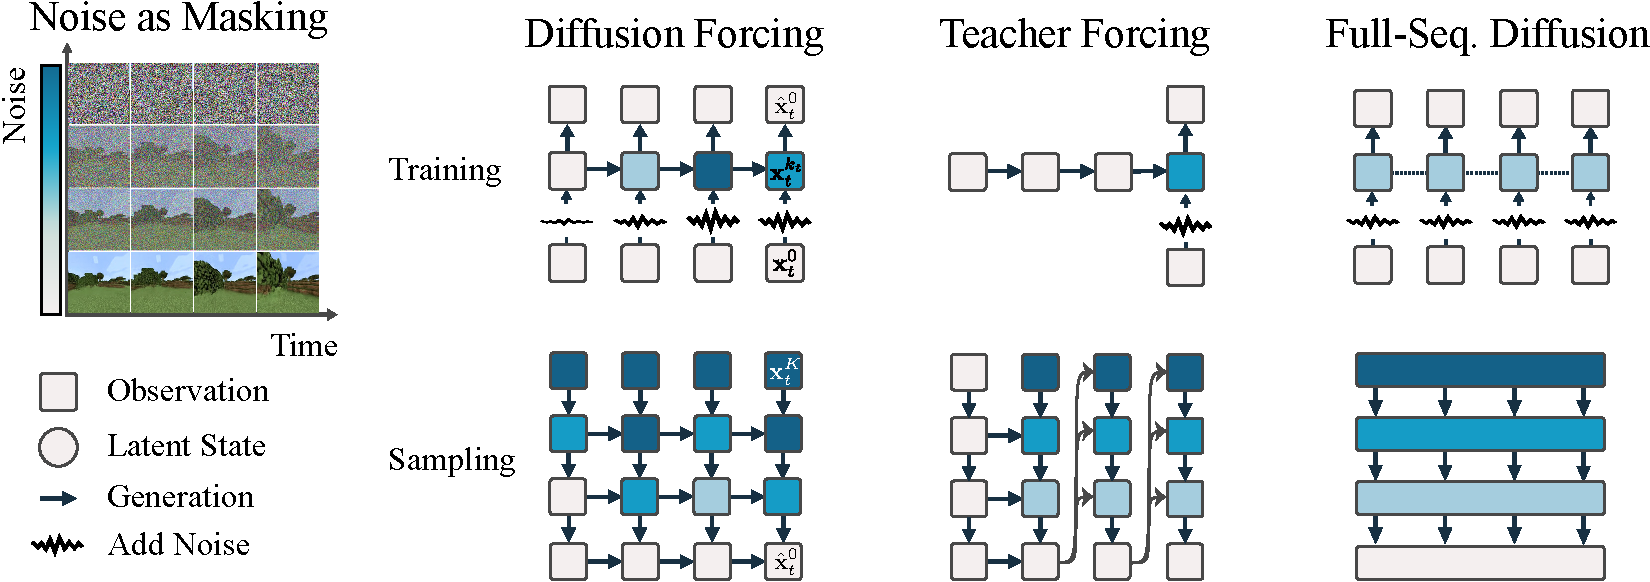
\includegraphics[width=\linewidth]{figures/pdf/Overview_best_guess.pdf}
    \caption{\textbf{Method Overview.} 
    Diffusion Forcing trains causal sequence neural networks (such as an RNN or a masked transformer) to denoise flexible-length sequences where each frame of the sequence can have a \emph{different} noise level.
    In contrast, next-token prediction models, common in language modeling, are trained to predict a single next token from a \emph{ground-truth} sequence (teacher forcing~\cite{teacher_forcing}), and full-sequence diffusion, common in video generation, train non-causal architectures to denoise all frames in a sequence at once with the \emph{same} noise level.
    \algo{} thus \emph{interleaves} the time axis of the sequence and the noise axis of diffusion, unifying strengths of both alternatives and enabling completely new capabilities (see Secs.~\ref{sec:zigzag_example},\ref{sec:method_decision_making}).
    }
    \label{fig:method}
    \vspace{-5pt}
\end{figure*}
 %Overview has been integrated in the introduction
\section{The \tool DSL}
\label{sec:dsl}
The \tool DSL extends the data representation in existing machine learning frameworks and provides constructs to express both computation and communication. 
The \tool DSL is embedded in C++.
Unifying the expression of computation and communication for distributed machine learning in the same DSL is the foundation to enable optimizations across computation and communication.

In this paper, we follow the MPI~\cite{mpi} terminology: \texttt{RANK} is the process ID of a distributed process, \texttt{GROUP} is a set of concurrent distributed processes, and \WORLD is the \texttt{GROUP} that includes all processes.
\tool supports dividing consecutive ranks into one or more process groups.

\begin{figure}[t]
  \footnotesize
%  \begin{subfigure}{0.49\textwidth}
  \begin{lstlisting}[language=DSL]
Tensor w(FP16, [H,H], Sliced(0), WORLD, RANK); |\label{line:mp:inputensor-begin}||\label{line:mp:continuous-tensor}|
Tensor b(FP16, [H], Replicated, WORLD); |\label{line:mp:inputensor-end}| 
Tensor in(FP16, [B,S,H], Sliced(2), WORLD, RANK);
Tensor r(FP16, [B,S,H], Replicated, WORLD);

// layer(FP16, [B,S,H], Local, WORLD, RANK)
Var layer = MatMul(in, w); |\label{line:mp:matmul}|
// sum(FP16, [B,S,H], Replicated, WORLD)
Var sum = AllReduce("+", layer); |\label{line:mp:allreduce}|
// dropout(FP16, [B,S,H], Replicated, WORLD)
Var dropout = Dropout(sum + b, 0.1); |\label{line:mp:pointwise-start}|
// out(FP16, [B,S,H], Replicated, WORLD)
Var out = dropout + r;|\label{line:mp:pointwise-end}|

Execute self_attention({w,in,b,r}, {out});
\end{lstlisting}
	\caption{An example program in \tool. \newline
		(\texttt{B}: batch size, \texttt{S}: sequence length, \texttt{H}: hidden dimension size)
	}
  \vspace{-2em}
    \label{fig:traditional-mp}
\end{figure}

\subsection{Tensor Layout}
\tool extends the concept of a tensor in machine learning frameworks from a single device data into distributed forms.
Besides item datatype, like \texttt{FP32} and \texttt{FP16}, and shape,
a \tool tensor also includes a \emph{layout} that describes the distributed allocation of tensor's data across a set of ranks. 
There are three layouts for a tensor: \emph{sliced}, \emph{replicated}, and \emph{local}.
A \emph{sliced} tensor is equally distributed among all nodes in a group along a specified dimension with \texttt{RANK} identifying the slice for that process.
% (first dimension by default). 
For example, in Figure~\ref{fig:traditional-mp}, which describes the Megatron-LM~\cite{megatronlm} model parallel logic of Self-Attention layer in \tool, \texttt{w} is sliced among all ranks in \WORLD in the 
first dimension and \texttt{in} is sliced in the third dimension.
A tensor can also be \emph{replicated} across all ranks in a group where it has the same value on each rank and it does not have a rank identifier.
For example, the bias \texttt{b} and the residual connection \texttt{r} are replicated as shown in Figure~\ref{fig:traditional-mp}. 
A \emph{local} tensor has same shape on all ranks but different
values on all ranks. A local tensor requires \texttt{RANK} to 
identify the values. For example, in Figure~\ref{fig:traditional-mp}, \texttt{layer}
is a local tensor that represents the result of MatMul operation.
A \texttt{Scalar} is a zero-dimensional tensor that represents a variable available on all ranks.
We discuss the layout of 
intermediate tensors in the next section.

\subsection{\tool's Operations}
A \tool program inherits the concept of data-flow graph (DFG) from existing machine learning frameworks with operations as vertices and data dependencies as edges.
Operations in \tool can be classified as (i) local computations, such as pointwise computations, matrix multiplication, and convolution, and (ii) cross rank communication operations, such as \allreduce, \allgather, and P2P \send-\recv.
%\tool follows numpy broadcast semantics and operation includes a matrix and a vector~\cite{numpymvm} \sm{this didn't make sense}.
Table~\ref{tab:operations} shows all operations supported by \tool{}.

A \texttt{Var} represents the intermediate tensor obtained after performing an operation. 
In the example of Figure~\ref{fig:traditional-mp}, the linear layer's weight (\texttt{w}) and the input
(\texttt{in}) are sliced across all ranks while the bias (\texttt{b}) and residual
(\texttt{r}) are replicated on all ranks. A \texttt{Var}'s shape and distribution layout are 
inferred based on the operation and inputs to the operation. For example,
line~\ref{line:mp:matmul} performs a MatMul operation on the input (\texttt{in}) and weights (\texttt{w}).
Since MatMul between two sliced tensors produces a local tensor, \texttt{layer} represents the partial result with \textit{local} layout.
At line~\ref{line:mp:allreduce}, \allreduce computes the sum of \texttt{layer} of all ranks and returns a \textit{replicated} tensor with the same values on each rank.
The computations at lines~\ref{line:mp:pointwise-start}--\ref{line:mp:pointwise-end} add the bias, use dropout as an activation, and add the residual. 
%Note that \texttt{b} and \texttt{sum} have shapes \texttt{[H]} and \texttt{[B,S,H]}, respectively.
At line~\ref{line:mp:pointwise-start}, the addition of \texttt{sum} and \texttt{b} follows
PyTorch's broadcast semantics\footnote{https://pytorch.org/docs/stable/notes/broadcasting.html} by replicating \texttt{b} in all dimensions of \texttt{sum}. 
Thus, the shape and layout of output of these operations are same as \texttt{sum}.
Finally, \texttt{Execute} defines the name, inputs, and outputs of the program. 

\begin{table}
  \small
  \caption{Operations supported by \tool includes all common communication and computation operations. \label{tab:operations}}
  \begin{tabular}{|c|l|}
    \hline
    \textbf{Communication} & AllReduce, AllGather, ReduceScatter, \\
    \textbf{Operations}    & Reduce, Broadcast, P2P Send-Recv \\\hline
    \textbf{Layers} & Matrix Multiplication, Convolution\\ \hline
    \textbf{Activations} & Dropout, tanh, ReLU \\ \hline
    \textbf{Tensor} & $+$, $-$, $*$, $\div$, Norm, ReduceTensor,\\
    \textbf{Operations} & Sqrt, Pow, Update\\\hline 
  \end{tabular}
  \par \bigskip% Do not remove this. Without this there is no space between the caption and the table
\end{table}

% In {\tool}, an input {\tt Tensor} has its distributed property tagged as \Sliced or \Replicated by user. 
% A \texttt{Var} has its distributed property and shape inferred from the operation producing it.
% For example, in \emph{MatMul} operation in Figure~\ref{fig:traditional-mp}, \texttt{layer}'s shape is [B, S, H] and exists locally (without any distribution information) as the sliced dimension in input tensors has vanished after computation. 
% %\TODO{or in \emph{Partial} property?}
% And according to the definition of \allreduce communication, \texttt{sum} is \replicated as the output is replicated across ranks. 
% %\sm{what is a tag? this paragraph is rough}

\subsection{Fused Collective Communication Operations}
\label{sec:fuse-comm-coll}
\tool enables efficient computations on the output of communication by providing fused collective communication operations, such as FusedAllReduce.
% To enable efficient computations on the output of communication, \tool extends all communication collectives to  fused communication collectives, such as FusedAllReduce.
Consider the \allreduce in Figure~\ref{fig:traditional-mp} followed by a Dropout (lines ~\ref{line:mp:allreduce}--\ref{line:mp:pointwise-start}).
The abstraction in existing machine learning frameworks requires the output of \allreduce 
to be stored in memory and then re-loaded by Dropout.
FusedAllReduce avoids such stores and loads by directly passing the output of communication to following computations through registers.
In addition to the argument of \allreduce, a FusedAllReduce takes computations as extra arguments.
Section~\ref{sec:code-gen-fused} discusses the implementation of Fused Collective Communication Operations.

\subsection{Overlapping Operations}
\label{sec:overlap-comm-coll}
\tool supports overlapping multiple dependent computation and communication operations using the \texttt{Overlap} construct.
For example, consecutive MatMul and \allreduce in Figure~\ref{fig:traditional-mp} 
(lines~\ref{line:mp:matmul}--\ref{line:mp:allreduce}) can be overlapped to fully utilize both network and computation resources.
Section~\ref{sec:overlap-impl} discusses the implementation of this construct.

\subsection{Custom Operations}
In \tool, the implementation of an operator needs to define three key properties of the operator: (i) syntax, (ii) semantics, and (iii) code generation.
The syntax of an operator is defined using C++ constructors and the semantics are defined by implementing rules to describe the layout and size of the output tensor based on the input tensors.
% This implementation of semantics is also used to validate the transformations.
Finally, the code generation requires implementing a function to generate a call to existing libraries or generate fused GPU kernels.
The implementation of syntax and semantics can be achieved in a few lines of code, however, implementing the code generation for complex operations like Matrix Multiplication and Convolution can potentially take hundreds of lines of code.
Fortunately, in practice the code generation for complex operations can call an optimized implementation of existing libraries.


\iffalse
\subsection{Communication Collectives}
\TODO{may move to section implementation}
In addition to the \allreduce primitive mentioned above, communication libraries like NCCL~\cite{nccl}, 
support several collective communications based on the MPI standard~\cite{mpi}. 
%NVIDIA Collective Communication Library~\cite{nccl} (NCCL) is a communication library for NVIDIA GPUs.
%NCCL provides communication primitive such as send and recv, and communication collectives to communicate between NVIDIA GPUs.
%Moreover, these functions follows MPI standards~\cite{mpi} and terminology.
%In the rest of the paper, 
The communication collectives in NCCL 
%NCCL provides five communication collectives and each 
take an input buffer $b_i$ of size $N_i$ and writes to an output buffer $b_o$ of size $N_o$.
\emph{\allreduce} performs a reduction operation on $b_i$ and leaves identical copies of $b_o$ on all ranks.
\emph{\allgather} gathers all $N_i$ values of $b_i$ from all ranks to $b_o$, such that, $N_o = N_i \times |\WORLD|$.
\emph{\reducescatter} performs a reduction operation on $b_i$ and scatter the result among all ranks in $b_o$, such that, $N_o = N_i \div |\WORLD|$.
\emph{\reduce} takes a root rank $r$ and performs reduction on $b_i$ and only writes the result to $b_o$ of $r$.
\emph{\broadcast} takes a root rank $r$. It copies $N_i$ values of $b_i$ of rank $r$ and leaves identical copies in $b_o$ of all ranks.
\fi

\iffalse 

%\paragraph{Example Tranformations}
\subsection{Equivalent Programs using Transformations}
\sm{this subsection provides nothing, I say we remove it.}
The way to express the same algorithm in \tool DSL is not unique.
%Previous work~\cite{mariannmt,zero,gshard} has observed that distributing the computation among ranks leads to better performance and lower memory usage for large models.
%These works 
For example, as shown in Figure~\ref{fig:reducescatter}, existing works~\cite{zero,gshard} distributes the computation by first doing \reducescatter to divide the summed values among all rank, then perform computation on the divided tensor, and finally performs \allgather to share the output of computation.
%as shown in Figure~\ref{fig:reduce-scatter-sgd}.
%Figure~\ref{fig:reduce-scatter-sgd} shows this optimization applied to model parallel update.
%While a user can specify this directly, the goal of \tool is to enable the transformations from Figure~\ref{fig:traditional-mp} to Figure~\ref{fig:reduce-scatter-sgd} and vice-versa through the scheduling language described in Section~\ref{sec:schedule}. 
Next section describes several output-invariant transformation between different concrete programs.
\fi

% For example, in Figure~\ref{fig:reduce-scatter-sgd}
% the contents of \lstinline[language=DSL]{m_} contains the values of
% \lstinline[language=DSL]{m} after {\em (i)} executing its arguments and
% {\em (ii)} storing the result of that computation in \lstinline[language=DSL]{m}.

\iffalse
\tool performs operations on 1-dimensional arrays, we refer to as Tensors.
\tool supports two types of operations that takes one or more tensors as input and returns one tensor.
First type is computations. 
\tool supports pointwise computations, where $i^{th}$ element of the output depends on the $i^{th}$ element of inputs, and reductions over a tensor using \texttt{ReduceTensor} construct.
Moreover, \tool supports casting of one element type to another.
This casting is useful for several scenarios like mixed precision training.
Second type are communication collectives supported by NCCL~\cite{nccl}.
A program written in \tool forms a Directed Acyclic Graph (DAG) of stages, where each \emph{stage} performs one or more computations and stage represent the output of the computation.
The properties of a stage, such as the size in each dimension, element type, are determined using the semantics of the computation.

Figure~\ref{fig:traditional-sgd} implements  Adam in \tool.
Tensors input to the program, such as gradient and weight, are defined 
using the \texttt{Tensor} (lines~\ref{line:adam:inputensor-begin}--\ref{line:adam:inputensor-end}).

Each tensor has four properties associated with it:
\begin{enumerate}
        \item \textbf{Element Type} of the tensor, such as, integers and floats.
        \item \textbf{Size}, i.e., the number of elements in the tensor.
        %  Currently \tool only supports single dimension tensors. However, we have found that this restriction does not prevent \tool from supporting a wide range of applications.
        \item \textbf{Set of Ranks} that stores this tensor in their memory. 
        A special set \WORLD contains all ranks.
        \item \textbf{Layout} \tool supports three layouts of a tensor.
        A \emph{\complete{}} tensor of size $N$ is stored on one or more ranks in a memory location of $N$ elements.
        A \emph{\replicated} tensor is a complete tensor that is stored on all ranks in \WORLD with each rank containing same contents.
        Since a \replicated tensor is a special kind of \complete tensor, \tool allows conversion of \replicated tensor to a \complete tensor.
        A \emph{\sliced{}} tensor of size $N$ stored on all ranks in \WORLD, is equally distributed among all ranks, such that, $i^{th}$ rank stores the $i^{th}$ part of tensor.
\end{enumerate}


Single dimension tensors that are input to the program and are available on all ranks are represented using \texttt{Scalar}.
Line~\ref{line:adam:scalars} defines \texttt{lr}, \texttt{beta1}, \texttt{beta2} as variables.
Each communication collective returns a \texttt{Stage} object. 
Lines~\ref{line:adam:avg} uses \allreduce to do elementwise reduction by summing all $i^{th}$ elements of \texttt{g} stored on all ranks and uses \texttt{avg} to represent the mean of these values.
Pointwise computations involving arithmetic, comparison, and bitwise operators can be expressed in a natural manner.
Pointwise computations are valid only when either both tensors are of same size and have same layout because operation is done on corresponding elements of both tensors, or when one or more tensor is a variable, hence, operation is done on the variable and each element of the tensor.
Lines~\ref{line:adam:pointwise-begin}--\ref{line:adam:pointwise-end} expresses pointwise computations to do the parameter update.
Finally, a \texttt{Pipeline} construct is used to define all inputs to the program and outputs of the program, which \tool uses to create the DAG stages.
\texttt{Pipeline::genCode} method generates CUDA code for all stages and links to NCCL API.
With default schedule, \tool generated code for  Adam is shown in Figure~\ref{fig:FusedSGD}.
% \paragraph{Tensor Functions}
% \tool provides two functions to retrieve a part of a tensor. First, the \texttt{at} function can be used to get an element at a particular index. Second, the \texttt{loadRank(Tensor\& t, int rank)} function returns the tensor stored at \texttt{rank}.
% \aj{I think a summary figure with all the above functions and their declarations will help? Or a figure with the grammar?}


% Addressed: \mm{Need to define {\it Continuous} tensors. I personally do not like the term Continuous, but its ok if we dont change it. Should we distinguish between Continuous tensors and "Replicated" tensors which have the same content in all nodes. AllReduce takes a Continuous Tensor and produces a Replicated Tensor. A Replicated Tensor {\it is a} Continuous tensor. We also need an operator that takes a Continuous tensor and produces a Tensor of a particular rank.}

\paragraph{Sliced Computations}

Many applications includes operation where $i^{th}$ rank performs computation on the $i^{th}$ part of the input to produce $i^{th}$ part of the output and then all parts of output can be combined using \allgather.
Recent techniques, such as Zero~\cite{zero}, utilizes this approach to do parameter update.
In \tool, we can express this algorithm as shown in Figure~\ref{fig:reduce-scatter-sgd}.
Lines~\ref{line:sliced-adam:inputensor-sliced-begin}--\ref{line:sliced-adam:inputensor-sliced-end} declares momentum and velocity tensors  
with the sliced layout.
At line~\ref{line:sliced-adam:reducescatter}, \reducescatter performs element-wise summation of gradient across the ranks to return a sliced stage.
Since momentum, velocity, and gradients are of sliced layout, we can perform all the pointwise computations.
However, before doing parameter update, we need to slice the parameters and then perform the computations(line~\ref{line:sliced-adam:sliced-parameter}).
Finally, an \allgather is introduced to gather all slices of updated parameters and store them in a \replicated layout (line~\ref{line:sliced-adam:allgather}).
\fi

%\tm{Describe update rule and relate to TF}


\iffalse

\subsubsection{Mixed Precisions}
% Mixed Precision neural network training~\cite{} is widely used to improve the training time.
% This technique involves computing gradients in 16-bit Half Precision Float, while parameters and other intermediates are stored in 32-bit Single Precision Float. 
% Using 16-bit Floats decreases the storage requirement and improves speed due to special computation that accelerates computation on 16-bit Floats, like Tensor Cores~\cite{}.
% \aj{Move above lines to background?}

\tool supports mixed precision applications where tensors can be of different type using its \texttt{Cast} construct, which cast all elements of the tensor to other type.
For example, in a parameter update that takes parameters in 32-bit Floats but gradients in 16-bit Floats, a \texttt{Cast} computation on gradients will cast all gradients from 16-bit Floats to 32-bit Floats.

\subsubsection{Tensor Reduction}
Many applications requires a reduction over tensors, such as, calculating the norm. 
For example, LAMB Optimizer~\cite{} calculates the norm of parameters and uses this norm in the parameter update. 
\tool provides \texttt{ReduceTensor} construct to perform a reduction computation on a tensor.
\texttt{ReduceTensor} supports several reduction operators, such as, sum, max, min.
\texttt{ReduceTensor} supports performing reduction on both \complete and sliced tensors and outputs a \texttt{Stage} containing a single element.
\fi

% \subsection{Model Parallelism in \tool}
% We now present the implementation of two widely used neural network optimizer Adam and LAMB in \tool.
% \aj{I think we should also have model parallelism here.}



\iffalse
\subsection{\tool's Functional Primitives}
\aj{probably needs to be removed}
\label{sec:functional-prmitives}
\newcommand{\List}[1]{\textit{List}[#1]}
\newcommand{\RepList}[1]{\textit{RepList}[#1]} 
\newcommand{\SlicedList}[1]{\textit{SlicedList}[#1]}
\newcommand{\LocList}[2]{\textit{LocList}_{#2}[#1]}
\newcommand{\func}[2]{#1 \rightarrow #2}
\newcommand{\lift}{\textit{lift}}
\newcommand{\funcdef}[3]{#1(#2) \rightarrow #3}

Given a program in \tool's DSL described above, \tool translates to a set of functional primitives. This provides a unified abstraction for computation and communication allowing us to define rewrite rules for transformations, validating the program using type checking rules, and generating code. 

We start with standard functional primitives. Starting with the base definition of $\List{T}$ as a vector of some type $T$, we define a tensor of $n$ dimensions recursively as a list of tensors of $n-1$ dimensions. Thus, a matrix is of type $\List{\List{T}}$ and so on. 
The function $\funcdef{map}{f:\func{T}{S}, l:\List{T})}{\List{S}}$ applies the function $f$ elementwise to the input list $l$. 
The function $\funcdef{fold}{l:\List{T}, f:\func{S\times T}{S}, a:S}{S}$ starts with the initial value $a$ and iteratively updates $a$ with $f(a,i)$ for each element $i$ in $l$. When $f$ is associative, we use $reduce$ instead of $fold$ to explicitly capture its parallel semantics.
 Another useful function is $zip$ that converts a pair of lists into a list of pairs. Also, we assume a $transpose$ function that permutes the dimension of a given tensor.   
We represent $map(f:\func{T}{S})$ as the `curried' version of $map$ that applies $f$ to an input $\List{T}$ and returns a $\List{S}$. Similarly, we use $\lift(f:\func{T\times S}{U})$ as the `zipped' version of the function that takes in a $\List{T}$ and $\List{S}$ and applies $f$ elementwise to return a $\List{U}$. For example, $\lift(+)$ represents vector addition, which allows us to define vector reduction as $reduce(lv: \List{\List{T}}, \lift(+), 0)$.

A key contribution of this work is to extend these functional primitives to work seamlessly
with distributed tensors. A $\RepList{T}$ represents a replicated tensor and a $\SlicedList{T}$ represents a sliced tensor. We also allow a tensor to be located at a particular rank $r$ with $\LocList{T}{r}$, with the function $rank$ returning the rank of such a list. Now we define primitives on these distributed tensors. 

The function $slice$ distributes a tensor along its first dimension to all the ranks in the \WORLD resulting in a sliced tensor. The function $join$ is its inverse. Similarly, the function $repl$ replicates a tensor to all the ranks in the \WORLD resulting in a replicated tensor, while $drop$ is its inverse. 
Finally, the function $store$ places a tensor at a particular rank, while $load$ removes this association. 
\begin{center}
$
\begin{array}{l}
\funcdef{slice}{l: \List{T}}{\SlicedList{T}}\\
\funcdef{join}{sl: \SlicedList{T}}{\List{T}}\\
\funcdef{repl}{l: \List{T}}{\RepList{T}}\\  
\funcdef{drop}{sl: \RepList{T}}{\List{T}}\\
\funcdef{store}{l: \List{T}, r: Int}{\LocList{T}{r}} \\
\funcdef{load}{ll: \LocList{T}{r}}{\List{T}}
\end{array}
$
\end{center}

These primitives allow us to capture the tensor computations and communication that occur in a distributed ML program. The base functional primitives allow us to capture tensor computations. For example, pointwise computations can be captured with $map$, dot product of two vectors with pointwise multiplication followed by a $reduce$, matrix-vector multiplication as a sequence of dot products, and so on. 

Lastly, our extensions for distributed tensors capture common communication collectives as shown below. 
These use the $reduce$ function on at least two dimensional sliced tensor.
$$\funcdef{reduce}{sl: \SlicedList{T}, f : (T \times T \rightarrow T)}{\List{T}}$$

\begin{figure}[H]
$
\begin{array}{l@{}l}
\text{Reduce}(sl: \SlicedList{T}, f, r) &: store(reduce(sl, f), r)\\
\text{Broadcast}(ll: \LocList{T}{r}) &: repl(load(ll))\\
\text{AllReduce}(sl: \SlicedList{T}, f) &: repl(reduce(sl, f))\\
\text{ReduceScatter}(sl: \SlicedList{T}, f) &: slice(reduce(sl, f))\\
\text{AllGather}(sl: \SlicedList{T}) &: repl(join(sl))\\
\end{array}
$
\end{figure}

% \begin{table*}
%   \small
%   % \begin{subtable}{\textwidth}
%     \begin{tabular}[]{|l|l|l|l|l|}\hline
%       \reduce & $l : List[Vector[T]] \rightarrow (f: T \rightarrow T \rightarrow T) \rightarrow List[Vector[T]] $  & $store(reduce(l, f), r)$ \\ \hline
%       \broadcast & $l : List[Vector[T]] \rightarrow RepList[Vector[T]] $  & $repl(l)$ \\ \hline
%       \allreduce & $l : List[Vector[T]] \rightarrow (f: T \rightarrow T \rightarrow T) \rightarrow RepList[Vector[T]] $  & $repl(reduce(l, f))$ \\ \hline
%       \reducescatter & $l : List[Vector[T]] \rightarrow (f: T \rightarrow T \rightarrow T) \rightarrow SliceList[Vector[T]] $ & $slice(reduce(l, f))$ \\ \hline
%       \allgather&$l : SliceList[Vector[T]] \rightarrow RepList[Vector[T]] $ & $repl(join(l))$ \\ \hline
%       TensorReduce & $l : RepList[Vector[T]] \rightarrow (f: Vector[T] \rightarrow T) \rightarrow RepList[T] $  & $repl(fold(head(l), f))$ \\ \hline
%       SlicedTensorReduce & $l : SlicedList[Vector[T]] \rightarrow (f: Vector[T] \rightarrow T) \rightarrow RepList[T] $  & $repl(fold(join(l), f))$ \\ \hline
%       Pointwise Function & $l: List[Vector[T]] \rightarrow (f: T \rightarrow T)$ & $map(map(f), l)$ \\ \hline
%       SlicedPointwise Function & $l: SliceList[Vector[T]] \rightarrow (f: T \rightarrow T)$ & $map(map(f), l)$ \\ \hline
%     \end{tabular}
%   \caption{\tool's constructs can be expressed using functional primitives\label{tab:constructs-to-primitives}}
% \end{table*}

% \begin{table*}
%   \small
%   % \begin{subtable}{\textwidth}
%     \begin{tabular}[]{|l@{}l|l|l|l|}\hline
%       \reduce & $:(l: \mathbf{List}, f: \mathbf{Op_r}, r: \mathbf{Int}) \rightarrow \mathbf{List}$ & $store(reduce(l, f), r)$ \\ \hline
%       \broadcast& $:(l: \mathbf{List})\rightarrow \mathbf{List}$ & $repl(l)$ \\ \hline
%       \allreduce& $:(l: \mathbf{List}, f: \mathbf{Op_r}) \rightarrow \mathbf{RepList}$ & $repl(reduce(l, f))$ \\ \hline
%       \reducescatter& $:(l: \mathbf{List}, f: \mathbf{Op_r}) \rightarrow \mathbf{SliceList}$&$slice(reduce(l, f))$ \\ \hline
%       \allgather&  $:(l: \mathbf{SliceList}) \rightarrow \mathbf{RepList}$& $repl(join(l))$ \\ \hline
%       TensorReduce& $:(l: \mathbf{RepList}, f: \mathbf{Op_r}) \rightarrow \mathbf{RepList}$ & $repl(fold(head(l), f))$ \\ \hline
%       Sliced TensorReduce& $:(l: \mathbf{SliceList}, f: \mathbf{Op_r}) \rightarrow \mathbf{RepList}$ &  $repl(fold(join(l), f))$ \\ \hline
%       Pointwise & $:(l: \mathbf{List}, f: \mathbf{F})\rightarrow \mathbf{List}$ & $map(map(f), l)$ \\ \hline
%       Sliced Pointwise& $:(l: \mathbf{SliceList}, f: \mathbf{F}) \rightarrow \mathbf{SliceList}$ & $map(map(f), l)$ \\ \hline
%     \end{tabular}
%   \caption{\tool's constructs can be expressed using functional primitives.
%   $List, SliceList$ and $RepList$ represents $List[Tensor[T]], SliceList[Tensor[T]]$ and $RepList[Tensor[T]]$ respectively.
%   $Op_r$ is type of a reduction function, i.e., $T \to T \to T$ and $F$ is type of a pointwise function, i.e., $T \to T$.
%   \label{tab:constructs-to-primitives}}
% \end{table*}
\fi

% \aj{Redo. Include stuff for Matmul}

%\subsection{Computation Validation}
%\label{sec:type-checking}
%\aj{Redo. Include stuff for Matmul}
%\tool performs validity of algorithm using \textit{static} checks on the functional primitives and generates \textit{dynamic} checks for the functional primitives representation.
%After converting the algorithm to functional primitives, the static checks are performed using the types of each primitive. 
%For example, $join$ takes a $SlicedList[T]$ as an argument and hence throws a type error if it is performed on a $LocList_r[T]$.
%Dynamic checks are generated to ensure that the rank parameter for $reduce$ is always in \WORLD and $load$ operation on $LocList_r[T]$ is valid when rank $r$ is in \WORLD.
%\tool generates code for these checks that uses a bit-vector representation of \WORLD.



\begin{figure*}[t]
	\centering
  %https://docs.google.com/drawings/d/1hXY1fwvREalsi9JpvJYvry8uEycz2XQH5jfAyFuhyJs/edit
  \includegraphics[width=\linewidth]{figures/coconet-example.pdf}
  \caption{\tool programs produced by performing transformations on the program of Figure~\ref{fig:traditional-mp}. Each schedule can be represented as a standalone program. Lines in \textcolor{red}{red} highlights changes at a step. (\texttt{AR}: AllReduce, \texttt{AG}: AllGather, and \texttt{RS}: ReduceScatter)
%  	to the program produced after applying the transformation.
  	\label{fig:mp-schedules}}
    \vspace{-1em}
\end{figure*}

\section{\tool Transformations}
\label{sec:schedule}
\tool provides four semantics preserving \emph{transformations} to optimize a program written in the DSL.
All transformations are valid based on rules described in the sections below. 
\tool automatically checks the validity of each transformation based on these rules and throws an error for  an invalid transformation.

We call an order of transformations a \emph{schedule}.
A user can manually specify the schedule to optimize the program.
Additionally, a user can invoke the autotuner to automatically find the best performing schedule for the given problem sizes and the underlying architecture.
Below we present each transformation by applying them on the program from Figure~\ref{fig:traditional-mp} and show equivalent \tool{} programs generated after applying each transformation in Figure~\ref{fig:mp-schedules}.

\subsection{Splitting Communication}
The \texttt{split} transformation breaks a collective communication operation into two communication operations.
One of the two split policies supported by \tool is

\textbf{AllReduce Split RS-AG} splits an \allreduce into a \reducescatter to produce a \sliced tensor and an \allgather on the \sliced tensor to return a \replicated tensor.

% \textbf{AllReduce Split B-R} splits an \allreduce into a \reduce to produce a tensor on user specified root rank and then \broadcast this tensor to all ranks in \WORLD.

\spara{Running Example} The \allreduce in Figure~\ref{fig:traditional-mp} is split into \texttt{rsSum} that does a \reducescatter on \texttt{layer} and \texttt{agSum} that does an \allgather on \texttt{rsSum}.
{
\small
\begin{lstlisting}[language=DSL,numbers=none]
(rsSum, agSum) = split(layer, ARSplitRSAG);
\end{lstlisting}
}

The program \circled{1} of Figure~\ref{fig:mp-schedules} is the implementation of this schedule where the input to Dropout is replaced by \texttt{agSum}.

\spara{\textit{Validity}} Since an \allreduce can always be split to a \reducescatter and an \allgather, this transformation is always valid.

\begin{figure}[t]
	\centering
	\includegraphics[width=.9\linewidth]{figures/reduceScatter}
%	\caption{Example of parallel Self-Attention layer on two GPUs using AllReduce (on left) and using ReduceScatter + AllGather (on right).}
	\caption{Equivalent programs (from Figure~\ref{fig:traditional-mp}) using AllReduce (on left) or using ReduceScatter + AllGather (on right).}
	\label{fig:model-parallel-using-reducescatter}
\end{figure}

\subsection{Reordering Operations}
The \texttt{reorder} transformation swaps operations with an \allgather or a \broadcast in the DFG of a program.
We explain this transformation for \allgather below: 

\textbf{AllGather Reorder} reorders an \allgather with communication and computation operations. 
This transformation changes the layout of the operations, the input and output of operations, and the input and output of the \allgather.
We explain this transformation below using the running example.

% \textbf{Broadcast Reorder} is similar to \allgather reorder except that it requires the user to specify a root rank.

\spara{Running Example}
In Figure~\ref{fig:mp-schedules}, applying the \texttt{reorder} transformation changes the program \circled{1} to \circled{2} by reordering \allgather (\texttt{agSum}) with computations \texttt{d} and \texttt{out}.
The reorder transformation replaces these operations in the DFG with three new operations: \texttt{scD} and \texttt{scOut},
both of which performs sliced computations, and \texttt{agOut}, which gathers the final result of computations.
{
  \small
\begin{lstlisting}[language=DSL,numbers=none]
(scD, scOut, agOut) = reorder(d, out, agSum);
\end{lstlisting}
}
The new sliced computations perform the same operations as original computations with two differences: (i) the output of \allgather used in the computation is replaced by the input of \allgather, and (ii) since the input of \allgather is sliced, 
all tensors input to the computations are also sliced along the same dimension as the input of \allgather.
After reorder, \texttt{scD} performs the same computation as \texttt{d} but \texttt{scD} takes \texttt{rsSum} and \texttt{Slice(r)} as input.
Therefore, the layout of \texttt{scOut} is also sliced while the computation is same as \texttt{out}.
Furthermore, the new \allgather is performed on the outputs of the computations, for example, 
after reorder, the \allgather (\texttt{agOut}) is performed on \texttt{scOut}.
Figure~\ref{fig:model-parallel-using-reducescatter} shows the workflow of this schedule.
% Here the input to Dropout is now the output of \reducescatter (\texttt{rsSum}) and computations are performed on slice of residual (\texttt{r}) to produce a sliced output.
% Then, \allgather collects the sliced output to obtain a replicated output.
% The next section describes fusion of communication and computation. 

\spara{\textit{Validity}} The \texttt{reorder} transformation is valid only if operations being reordered with an \allgather can be sliced along the dimension the \allgather is performed.
The rules of slicing an operation depend on the type of operation and the dimensions of inputs to the operations.
For example, \texttt{d} and \texttt{out} can be sliced because the computations have the same dimensions as \texttt{agOut}.
Section~\ref{sec:opt-workloads} shows how P2P Send can be reordered with an \allgather.
% A MatMul can be sliced in the rows or columns dimension of the output matrix but not in the reduction dimension.

\subsection{Fusing Operations}
\label{sec:sched:fusion}

Fusing multiple computations is a common technique used by existing compilers~\cite{tvm18,distributed-halide,fireiron,polymage-gpu,halide}.
\tool extends this concept to fuse multiple computations and communications in a single operation and provides this capability using the \texttt{fuse} transformation.
Below we explain two fuse policies supported by \tool:

\textbf{Computation Fuse} fuses a series of computations in a single operation that performs all these operations.

\textbf{AllReduce Fuse} fuses a series of \reducescatter, sliced computations, and \allgather operations in a single Fused\allreduce that performs all these operations.

\spara{Running Example}
We can fuse \reducescatter (\texttt{rsSum}), computations (\texttt{scD} and \texttt{scOut}), and \allgather (\texttt{agOut}) in program \circled{2} of Figure~\ref{fig:mp-schedules} into a Fused\allreduce to obtain program \circled{3}.
{
\small
\begin{lstlisting}[language=DSL,numbers=none]
fuseAR = fuse(rsSum, scOut, agOut, ARFuse);
\end{lstlisting}
}
The \texttt{comp} method of \texttt{fusedAR} specifies the computation to be fused with Fused\allreduce and returned \texttt{out} is the output.

\spara{\textit{Validity}} Fusing multiple operations into one operation is valid only if the dependencies in the DFG after fusion are preserved.

\subsection{Overlapping Operations}
\tool provides the \texttt{overlap} transformation to overlap a series of producer-consumer operations to utilize multiple resources of hardware simultaneously.
% One use case of this transformation is to overlap computation and communication operations.
% It takes two or more operations as input and returns a single operation.

\spara{Running Example} 
In the program \circled{3} of Figure~\ref{fig:mp-schedules} we overlap the matrix multiplication (\texttt{layer}) with Fused\allreduce (\texttt{fuseAR}) to obtain program in \circled{5}.
{
\small
\begin{lstlisting}[language=DSL,numbers=none]
layerWithAR = overlap(layer, fusedAR);
\end{lstlisting}
}

\spara{\textit{Validity}} Overlapping multiple operations is valid only when all operations have a producer-consumer relationship between them.

% Operation returned by \texttt{Overlap} is the final output of the program.

\subsection{Automatic Exploration of Schedules}
\tool provides an \emph{autotuner} to automatically explore the space of all schedules of a program and return the schedule that provides the best performance for the underlying architecture and input sizes.
First, the autotuner fuses all pointwise computations up to a pre-defined threshold to decrease the search space and then exhaustively explores the schedule space in a breadth first search manner.
Finally, the autotuner generates code for all schedules in its search space, executes all programs, and returns the schedule with minimum execution time.
Table~\ref{tab:loc-autotuner-time} shows that the autotuner takes only a few seconds to explore the schedule space for all workloads.

\begin{figure}
  \small
  \centering
% Scalar lr(FP32), beta1(FP32), beta2(FP32);|\label{line:adam:scalars}|
% Tensor g(FP32, WORLD_SZ, SIZE, Sliced); |\label{line:adam:inputensor-begin}||\label{line:adam:continuous-tensor}|
% Tensor p(FP32, WORLD_SZ, SIZE, Replicated);
% Tensor m(FP32, WORLD_SZ, SIZE, Replicated);
% Tensor v(FP32, WORLD_SZ, SIZE, Replicated);|\label{line:adam:inputensor-end}| 
  \begin{subfigure}[t]{\columnwidth}
\begin{lstlisting}[language=DSL, numbers=left]
Var avg = AllReduce("+", g); |\label{line:adam:avg}|
Var m_ = Update(m, (m*beta1+(1-beta1)*avg));|\label{line:adam:pointwise-begin}||\label{line:update:m}|
Var v_ = Update(v, (v*beta2+(1-beta1)*avg*avg));|\label{line:update:v}|
Var m1 = m_/(1-Pow(beta1, t));
Var v1 = v_/(1-Pow(beta2, t));
Var p_ = Update(p, (p - lr * m1/(Sqrt(v1))));|\label{line:adam:pointwise-end}|

Execute adam({g,p,v,m,lr}, {p_});
\end{lstlisting}
\caption{Traditional implementation where 
               tensors \texttt{g} is local to each rank and \texttt{p},\texttt{m}, and \texttt{v} are replicated on all ranks.}
\label{fig:traditional-adam}
\end{subfigure}
\par\bigskip % Do not remove this. Without this there is no space between caption of above figure and the next figure. WEIRD bug. Never saw this in subfigure.
\begin{subfigure}[b]{\columnwidth}
\begin{lstlisting}[language=DSL, numbers=left]
comps = fuse(m_, v_, m1, v1, p_, 
             ComputationFuse);|\label{line:adam-schedule:fuse-comp}|
(rsG, agG) = split(avg, ARSplitRSAG); |\label{line:adam-schedule:split}|
(scComp, agP, agM, agV) = reorder(agG, comps, 
                                  AGReorder);|\label{line:adam-schedule:reorder}|  
asSlice(m); asSlice(v); dead(agM); dead(agV); |\label{line:adam-schedule:slice-m-v}| |\label{line:adam-schedule:remove-m-v-allgather}|
fuseAR = fuse(rsG, scComp, agP, AllReduceFuse);|\label{line:adam-schedule:fuse-allreduce}|
\end{lstlisting}
\caption{An Optimized Schedule. Tensors \texttt{g} is local, \texttt{p} is replicated on all ranks, while 
\texttt{m} and \texttt{v} are sliced among all ranks.}
\label{fig:adam-schedule}
\end{subfigure}
% Scalar lr(FP32), beta1(FP32), beta2(FP32);|\label{line:adam:scalars}|
% Tensor g(FP32, WORLD_SZ, SIZE, Sliced); |\label{line:adam:inputensor-begin}||\label{line:adam:continuous-tensor}|
% Tensor p(FP32, SIZE, Replicated);
% Tensor m(FP32, SIZE, Sliced);
% Tensor v(FP32, SIZE, Sliced);|\label{line:adam:inputensor-end}| 
% \hfill{}
% \begin{subfigure}{0.32\textwidth}
%   \begin{lstlisting}[language=DSL, numbers=left]
% avg = FusedAllReduce("+", g); |\label{line:adam:avg}|
% scP_ = p.update(p - scDiff);
% p_ = fuseAR.comp(scP_);

% adam({g,p,v,m,lr}, {p_});
%   \end{lstlisting}
% \caption{Equivalent \tool implementation after applying the schedule. 
% Tensors \texttt{g} and \texttt{p} are replicated on all ranks, while 
% \texttt{m} and \texttt{v} are sliced among all ranks. \texttt{scDiff}
% represents the sliced \texttt{diff}. \label{fig:optimized-adam}}
% \end{subfigure}
  \caption{Optimizing parameter update using Adam in \tool. 
  The implementation takes four input tensors: parameters (\texttt{p}), gradients (\texttt{g}),
  momentum (\texttt{m}), and velocity (\texttt{v}).
  \label{fig:optimizing-adam}}
  \end{figure}

\section{Distributed Workloads in \tool}
\label{sec:opt-workloads}
We additionally optimized two distributed machine learning workloads using \tool: (i) parameter update using Adam~\cite{adam}, and (ii) point-to-point communication in pipeline parallelism.

\spara{Adam in Data Parallel Training}: Figure~\ref{fig:traditional-adam} shows the traditional implementation of parameter update using Adam.
First, all ranks average the gradients using \allreduce and then perform computations to update the optimizer state and model parameters.
\texttt{Update} updates the values of a tensor and reflects the new values in that position in the DFG (lines~\ref{line:update:m}--\ref{line:update:v}).
Figure~\ref{fig:adam-schedule} presents a schedule that optimizes this by distributing the computation on all ranks in a single kernel.
Line~\ref{line:adam-schedule:fuse-comp} fuses all computations in \texttt{comps}.
Line~\ref{line:adam-schedule:split} splits the \allreduce into a \reducescatter and an \allgather, such that computations take output of \allgather (\texttt{agG}) as input.
Line~\ref{line:adam-schedule:reorder} reorders \allgather with computations, such that,
each rank performs computations on a slice of tensors.
% \allgather operations are returned for parameters and optimizer state.
Line~\ref{line:adam-schedule:slice-m-v} slices optimizer states on all ranks to decrease memory usage and removes corresponding \allgather.
Finally, line~\ref{line:adam-schedule:fuse-allreduce} fuses all operations in a single kernel.

\begin{figure}[t]
  \begin{subfigure}{\columnwidth}
  \centering
  \includegraphics[width=.85\linewidth]{figures/pipeline-p2p-fusion-1.pdf}  
  \caption{In Megatron-LM each GPU sends redundant data. \label{fig:p2p-fusion-1}}
\end{subfigure}
\par\bigskip % Do not remove this. Without this there is no space between caption of above figure and the next figure. WEIRD bug. Never saw this in subfigure.
\begin{subfigure}{\columnwidth}
  \centering
  \includegraphics[width=.85\linewidth]{figures/pipeline-p2p-fusion-3.pdf} 
  \caption{Communication operations can be overlapped at the granularity of each 
  \emph{communication buffer tile} of data in single kernel 
  call.\label{fig:p2p-fusion-3}}
\end{subfigure}
  \caption{Two different schedules of pipeline parallelism.
\label{fig:P2Ptimeline}}
\end{figure}

\spara{Point-to-Point Communication in Pipeline Parallelism}: 
Figure~\ref{fig:p2p-fusion-1} shows a scenario of pipeline parallelism in Megatron-LM
with two transformer layers assigned to two groups each with two ranks. 
Rank $i$ in group $j$ is shown by $(j,i)$.
Each group uses model parallelism within its transformer layer.
Pipeline parallelism in Megatron-LM works as follows.
First, all ranks in the first group reduce their input using 
\allreduce to get replicated output.
Then each rank performs pointwise computations over the replicated output.
Finally, the first group sends the result of computations to the corresponding rank in the
second group using point-to-point (P2P) sends. (Line~\ref{line:p2p:comp2} in Figure~\ref{fig:traditional-p2p} shows these computations but are omitted in Figure~\ref{fig:P2Ptimeline} for simplicity). Since the output of \allreduce in 
Figure~\ref{fig:p2p-fusion-1} is replicated, redundant data is sent using P2P.
We can avoid this redundant communication by splitting
the \allreduce to \reducescatter and \allgather and reordering the P2Ps with the
\allgather. 
Hence, the inter-group communication is reduced by 
the group size.
We can further optimize by overlapping all communication operations. 
Figure~\ref{fig:p2p-fusion-3} shows that if the 
buffers are split into multiple tiles (\texttt{T0}--\texttt{T2} in the figure), 
intra-group and inter-group communications can be overlapped.
%  to further reduce the communication time.

% Figure~\ref{fig:optimizing-p2p} shows how to do these 
% optimizations with \tool. 
Figure~\ref{fig:traditional-p2p} is the original program, 
while Figure~\ref{fig:p2p-schedule} optimizes it by applying transformations.
Line~\ref{line:p2p:fuse-send} fuses the P2P 
send with computations.
Line~\ref{line:p2p:split} splits the \allreduce and reorders the returned \allgather with the fused P2P send at Line~\ref{line:p2p:reorder}.
Hence, P2P send and computations are performed 
on only a slice of data on the next group where the \allgather is also performed.
Finally, all three new operations get overlapped in Line~\ref{line:p2p:fuseAR}.
% This overlapping can only be achieved by generating custom communication and computation kernels.
%Figure~\ref{fig:traditional-p2p} shows the implementation of pipeline parallelism in Megatron-LM.
%Here one Transformer layer is assigned to a group of consecutive ranks, such that each group uses model parallelism for the Transformer layer.
%First all ranks in a group perform reduces their input (\texttt{in}) using \allreduce to obtain a replicated output.
%Each rank in the group sends the output to same rank of next group using point-to-point (P2P) communication, over which several pointwise computations are done.
%Figure~\ref{fig:p2p-schedule} optimizes the program by avoiding send of redundant replicated output. 
%Lines~\ref{line:p2p:fuse-comp}--\ref{line:p2p:fuse-send} fuses the P2P send with computations.
%At line~\ref{line:p2p:reorder} \allreduce is split and the returned \allgather is reordered with fused send, so that, both P2P send and computations are performed on only a slice of data on the next group and the \allgather is also performed on the next group.
%Finally, all three new operations can be overlapped because \reducescatter and \allgather are performed in different groups and P2P send uses interconnect between the groups.

\begin{figure}[!t]
	\small
	\begin{subfigure}{\columnwidth}
		\begin{lstlisting}[language=DSL, numbers=left]
Var sum = AllReduce("+", in);
Var send = Dropout(recv+b,0.1) + r;|\label{line:p2p:comp1}||\label{line:p2p:comp2}|
Var output = Send(send, 
                  GroupRank(GROUP+1, RANK));

Execute transformer({in}, {output});
		\end{lstlisting}
		\caption{Traditional implementation. Each rank of a group sends same data to next group.}
		\label{fig:traditional-p2p}
	\end{subfigure}
	\par\bigskip % Do not remove this. Without this there is no space between caption of above figure and the next figure. WEIRD bug. Never saw this in subfigure.
	\begin{subfigure}{\columnwidth}
		\begin{lstlisting}[language=DSL, numbers=left]
fuseSend = fuse(send, output, SendFuse);|\label{line:p2p:fuse-send}|
(rsSum, agSum) = split(sum, ARSplitRSAG); |\label{line:p2p:split}|
(scSend, agOut) = reorder(fuseSend, agSum, 
                          AGReorder); |\label{line:p2p:reorder}|
overlapOut = overlap(rsSum, scSend, agOut); |\label{line:p2p:fuseAR}|
		\end{lstlisting}
		\caption{An Optimized Schedule. Each rank sends only a slice of data to ranks in next group and all operations are overlapped.}
		\label{fig:p2p-schedule}
	\end{subfigure}
	\caption{Optimizing pipeline parallelism of Megatron-LM. Input tensors: layer output \texttt{in}, bias \texttt{b}, and residual \texttt{r}. \label{fig:optimizing-p2p}}
\end{figure}


\iffalse

\begin{figure*}[t]
    \small
\begin{subfigure}{0.49\textwidth}
    \begin{lstlisting}[language=DSL]
    Variable lr(Float);
    Variable m(Float);
    Tensor g(Float, SIZE, GPUs);
    Tensor p(Float, SIZE, GPUs);
    Tensor v(Float, SIZE, GPUs);
    
    Stage sum = AllReduce("+", g);
    Stage v_ = m * v + sum/GPUs;
    Stage p_ = p - lr * v_;
    
    Pipeline pipeline({g, p, m, lr}, {v}, {p_});
\end{lstlisting}
\caption{Optimizing  SGD in \tool }
    \label{fig:traditional-sgd}
\end{subfigure}

\begin{subfigure}{0.45\textwidth}
\begin{lstlisting}[language=DSL]     
        Stage sumRS;
        Stage sumAG;
        pipeline.split(sum, &sumRS, &sumAG, 
                       ReduceScatterAllGather); 
\end{lstlisting}
\caption{}
\end{subfigure}
\begin{subfigure}{0.45\textwidth}
        \begin{lstlisting}[language=DSL]     
                sumRS = ReduceScatter(g); 
                sumAG = AllGather(sumRS)
                //Replace all references of 
                //sum with sumAG
        \end{lstlisting}
        \caption{}
\end{subfigure}

\begin{subfigure}{0.45\textwidth}
\begin{lstlisting}[language=DSL]     
        Stage v1_, vAG;
        pipeline.reorder(v_, sumAG, v1_, vAG); 
\end{lstlisting}
\caption{}
\end{subfigure}
\begin{subfigure}{0.45\textwidth}
        \begin{lstlisting}[language=DSL]     
                v1_ = m * slice(v) + sumRS/GPUs; 
                vAG = AllGather(v1_);
                p_ = p - lr * vAG;
        \end{lstlisting}
        \caption{}
\end{subfigure}

\begin{subfigure}{0.45\textwidth}
\begin{lstlisting}[language=DSL]     
        Stage p1_, pAG;
        pipeline.reorder(vAG, p_, p1_, pAG); 
        pipeline.asSlice(v); 
        pipeline.fuse({sumRS, v1_, p1_, pAG}, 
                      AllReduce); 
        pipeline.storeAt({p_, p},{v_, v});
\end{lstlisting}
\caption{}
\end{subfigure}
\begin{subfigure}{0.45\textwidth}
\begin{lstlisting}[language=DSL]     
        v1_ = m * slice(v) + sumRS/GPUs; 
        pAG_ = slice(p) - lr * v1_; 
        p1_ = AllGather(pAG_);
\end{lstlisting}
\caption{}
\end{subfigure}

\begin{subfigure}{0.45\textwidth}
\begin{lstlisting}[language=DSL]     
        pipeline.asSlice(v); 
        pipeline.fuse({sumRS, v1_, p1_, pAG}, 
                        AllReduce); 
        pipeline.storeAt({p1_, p},{v1_, v});
\end{lstlisting}
\caption{}
\end{subfigure}
\caption{SGD with momentum}
\end{figure*}



\begin{figure*}[t]
    \small
\begin{subfigure}{0.49\textwidth}
    \begin{lstlisting}[language=DSL]
    Variable lr(Float);
    Variable m(Float);
    Tensor g(Float, SIZE, GPUs);
    Tensor p(Float, SIZE, GPUs);
    Tensor v(Float, SIZE, GPUs);
    Tensor m(Float, SIZE, GPUs);
    
    Stage sum = AllReduce("+", g);
    Stage m_ = beta1 * m + (1-beta1)*sum;
    Stage v_ = beta2 * v + (1-beta2)*(sum*sum);
    Stage p_ = p - lr * m_/(1-beta1)/(sqrt(v_/(1-beta2)));
    
    Pipeline pipeline({g, p, m, lr}, {v}, {p_});
\end{lstlisting}
\caption{Optimizing  Adam in \tool }
    \label{fig:traditional-sgd}
\end{subfigure}

\begin{subfigure}{0.45\textwidth}
\begin{lstlisting}[language=DSL]     
        Stage sumRS;
        Stage sumAG;
        pipeline.split(sum, &sumRS, &sumAG, 
                       ReduceScatterAllGather); 
\end{lstlisting}
\caption{}
\end{subfigure}
\begin{subfigure}{0.45\textwidth}
        \begin{lstlisting}[language=DSL]     
                sumRS = ReduceScatter(g); 
                sumAG = AllGather(sumRS)
                //Replace all references of 
                //sum with sumAG
        \end{lstlisting}
        \caption{}
\end{subfigure}

\begin{subfigure}{0.45\textwidth}
\begin{lstlisting}[language=DSL]    
        Stage mv;
        pipeline.fuse({m_,v_}, mv) ;
        Stage mv_, mvAG;
        pipeline.reorder(mv_, sumAG, mv1_, mvAG); 
\end{lstlisting}
\caption{}
\end{subfigure}
\begin{subfigure}{0.45\textwidth}
        \begin{lstlisting}[language=DSL]     
                Stage m_ = beta1 * slice(m) + (1-beta1)*sumRS;
                Stage v_ = beta2 * slice(v) + (1-beta2)*(sumRS*sumRS);
                vAG = AllGather(v1_);
                mAG = AllGather(m1_);
                p_ = p - lr * f(mAG, vAG);
        \end{lstlisting}
        \caption{}
\end{subfigure}

\begin{subfigure}{0.45\textwidth}
\begin{lstlisting}[language=DSL]     
        Stage p1_, pAG;
        pipeline.reorder(mvAG, p_, p1_, pAG); 
        pipeline.asSlice(v); 
        pipeline.asSlice(m); 
        
\end{lstlisting}
\caption{}
\end{subfigure}
\begin{subfigure}{0.45\textwidth}
\begin{lstlisting}[language=DSL]     
        v1_ = m * slice(v) + sumRS/GPUs; 
        pAG_ = slice(p) - lr * v1_; 
        p1_ = AllGather(pAG_);
\end{lstlisting}
\caption{}
\end{subfigure}

\begin{subfigure}{0.45\textwidth}
\begin{lstlisting}[language=DSL]     
        pipeline.asSlice(v); 
        pipeline.fuse({sumRS, v1_, p1_, pAG}, 
                        AllReduce); 
        pipeline.storeAt({p1_, p},{v1_, v});
\end{lstlisting}
\caption{}
\end{subfigure}
\caption{Adam}
\end{figure*}


\begin{figure*}[t]
        \small
\begin{subfigure}{0.49\textwidth}
        \begin{lstlisting}[language=DSL]
        Variable lr(Float);
        Variable m(Float);
        Tensor g(Float, SIZE, GPUs);
        Tensor p(Float, SIZE, GPUs);
        Tensor v(Float, SIZE, GPUs);
        Tensor m(Float, SIZE, GPUs);
        
        Stage sum = AllReduce("+", g);
        Stage m_ = beta1 * m + (1-beta1)*sum;
        Stage v_ = beta2 * v + (1-beta2)*(sum*sum);

        Stage r1 = Reduce("+", p * p);
        Stage p_upd = m_ / sqrt(v_ + eps) + lambda * p
        Stage r2 = Reduce("+", p_upd * p_upd)

        Stage p_ = p - r1/r2*lr* p_upd
        
        Pipeline pipeline({g, p, m, lr}, {v}, {p_});
    \end{lstlisting}
\end{subfigure}
\caption{LAMB}

\begin{subfigure}{0.49\textwidth}
        \begin{lstlisting}[language=DSL]
        Variable lr(Float);
        Variable m(Float);
        Tensor g(Float, SIZE, GPUs);
        Tensor p(Float, SIZE, GPUs);
        Tensor v(Float, SIZE, GPUs);
        Tensor m(Float, SIZE, GPUs);
        Stage p_slc = slice(p)


        Stage sumRS = ReduceScatter("+", g);
        Stage m_slc = beta1 * slice(m) + (1-beta1)*sumRS;
        Stage v_slc = beta2 * slice(v) + (1-beta2)*(sumRS*sumRS);
        Stage p_upd_slc = m_slc / sqrt(v_slc + eps) + lambda * p_slc

        Stage r1 = AllReduce("+", p_slc * p_slc);
        Stage r2 = AllReduce("+", p_upd_slc * p_upd_slc)

        Stage p_slc_ = p_slc - r1/r2*lr* p_upd_slc

        Stage p_ = AllGather(p_slc_)

        Pipeline pipeline({g, p, m, lr}, {v}, {p_});
    \end{lstlisting}
\end{subfigure}

\caption{Optimizing LAMB in \tool }
        \label{fig:lamb}
\end{figure*}

\tool automatically checks validity of each computation based on a set of \emph{validation rules}.
Each validation rule checks the properties of all tensors involved in the computation and assign values to all properties of the output tensor.
Figure~\ref{fig:rules} presents the validation rules for all computations supported by \tool.
In the validation rules the four properties of a tensor (T) are represented as follows: (i) $\type{}$ is the type of elements, 
(ii) $n$ is the number of elements, (iii) $\Locs{}$ is the set of ranks, and (iv) $\alloc{}$ is the allocation type.
Below we explain the validation rules of all computations.

\paragraph{Pointwise Computations} Pointwise computations are valid only if the input tensors have same value of properties and the output tensor will have properties with these values (rules \textsc{E-BinaryOp} and \textsc{E-UnaryOp}).

\paragraph{Communication Collectives} Each computation involving a NCCL Communication Collective computations has a validation rule associated, which follows the semantics of the computation defined in the NCCL documentation~\cite{}.
\allreduce on the input tensor is valid only if the input is a \complete tensor and present on all ranks in the \WORLD (\textsc{E-AllReduce}). After \allreduce, the output tensor has same properties as the input tensor.
Similar to \allreduce, \reducescatter requires same conditions on the input tensor but the output tensor will be equally \sliced among all ranks in \WORLD (rule \textsc{E-ReduceScatter}).
Since \allgather gathers all slices from all ranks and stores these slices in \complete tensors on all ranks, \allgather requires input tensor to be a \sliced tensor stored on all ranks in \WORLD and the output tensor is a \complete (rule \textsc{E-AllGather}).
Slicing a tensor is possible only if it is continuous and the output tensor is stored on all ranks where the input tensor was stored (rule \textsc{E-Scatter}).
So far we have presented the validation rules that can be checked during the compile time.
However, the rules for allocation type for Reduce and Broadcast must be dynamically checked because both requires a particular rank as input, which must be checked at the runtime if it belongs to \WORLD.
These dynamic checks are automatically generated by \tool code generator (discussed in Section~\ref{sec:code-gen}).
\reduce can be called on tensors that are present on all ranks in \WORLD with the target rank in the \WORLD and the output tensor is available on the target rank only (rule \textsc{E-Reduce}).
On the other hand, Broadcast is valid only for \complete tensors and when all nodes in \WORLD will receive the output tensor(rule \textsc{E-Broadcast}).

\paragraph{LoadTensorAtRank}

\paragraph{ReduceTensor} Reducing a single tensor is possible on both \sliced or \complete tensors. However, the tensor must be stored on all ranks in \WORLD (rule \textsc{E-ReduceTensor}).
The output tensor will contain only one element, which will have different value for different ranks.

\paragraph{Cast} According to the validation rule \textsc{E-Cast} the  output tensor has same properties as the input tensor, except the output's element type is the argument of Cast.

\paragraph{Example} We illustrate type checking on \tool code in Figure~\ref{fig:FusedSGD} and Figure~\ref{fig:reduce-scatter-sgd}.
In Figure~\ref{fig:FusedSGD}, \allreduce produces a \complete stage of same size, element type, and on nodes.
Then the computations on lines~\ref{}--\ref{} again produces tensors with same properties. 
In contrast, Figure~\ref{fig:reduce-scatter-sgd} uses a \reducescatter to generate a tensor of size \aj{To be continued}

\begin{figure}[t]
  \small
\begin{subfigure}{\columnwidth}
\(
\begin{array}{@{}l@{}r@{\,}c@{\,}l@{}}
        \textbf{Tensors} & \tensor{}^{[\type{},n,\Locs{}, \alloc{}]}\\
        \text{Element Type} & \type{} & \in & \ldots\\ %\{u8, i8, f16, \cdots,  u64, i64, f64\} \\
        \text{Tensor Size} & n & \in & Z^{+} \\
        \text{Set of all ranks} & WORLD & \subseteq & Z^{+} \\
        \text{Set of Storage Locations} & \Locs{} & \subseteq & WORLD\\
        \text{Allocation Type} & \alloc{} & \in & \{\text{\complete, Sliced}\}\\
        \text{Pointwise Computations} & \texttt{op} & \in &{+, -, *, /, pow}\\
\end{array}
\)
\end{subfigure}

\begin{subfigure}{\columnwidth}
\begin{mathpar}
\inferrule*[Left=E-BinaryOp]
        {\tensor{}_{1}^{[\type{}_1,n_1,\Locs{}_1, \alloc{}_1]} = \texttt{op}(\tensor{}_{2}^{[\type{},n,\Locs{},\alloc{}]}, \tensor{}_{3}^{[\type{},n,\Locs{},\alloc{}]})}
        {\type{}_1 = \type{} \\ n_1 = n \\ \Locs{}_1 = \Locs{} \\ \alloc{}_1 = \alloc{}}\\ %\forall_{\loc{} \in \Locs{}}\forall_{0 \leq i \leq n} \tensor{}_{1}[\loc{}, i] = \texttt{op}(\tensor{}_{2}[\loc{}, i], \tensor{}_{3}[\loc{}, i])
\inferrule*[Left=E-UnaryOp]
        {\tensor{}_{1}^{[\type{}_1,n_1,\Locs{}_1, \alloc{}_1]} = \texttt{op}(\tensor{}_{2}^{[\type{},n,\Locs{},\alloc{}]})}
        {\type{}_1 = \type{} \\ n_1 = n \\ \Locs{}_1 = \Locs{} \\ \alloc{}_1 = \alloc{}}\\ %\forall_{\loc{} \in \Locs{}}\forall_{0 \leq i \leq n} \tensor{}_{1}[\loc{}, i] = \texttt{op}(\tensor{}_{2}[\loc{}, i], \tensor{}_{3}[\loc{}, i])
\inferrule*[Left=E-Slice]
        { {
          \begin{array}{ll}
            \tensor{}_{1}^{[\type{}_1,n_1,\Locs{}_1,\alloc{}_1]} = \texttt{Slice}(\tensor{}^{[\type{},n,\Locs{},\alloc{}]})\\
            \alloc{} = \complete
          \end{array}
        } }
        {
          {
            \begin{array}{ll}
              \type{}_1 = \type{} & n_1 = \frac{n}{|\Locs{}|} \\ 
              \Locs{}_1 = \Locs{} & \alloc{}_1 = \sliced
            \end{array}
          }
        }\\
\inferrule*[Left=E-Cast]
        {\tensor{}_{1}^{[\type{}_1,n_1,\Locs{}_1,\alloc{}_1]} = \texttt{Cast}(\tensor{}^{[\type{},n,\Locs{},\alloc{}]}, \type{}_2)}
        {\type{}_1 = \type{}_2 \\ n_1 = n \\ \Locs{}_1 = \Locs{} \\ \alloc{}_1 = \alloc{}}\\
\inferrule*[Left=E-LoadTensorAtRank]
        {\tensor{}_{1}^{[\type{}_1,n_1,\Locs{}_1,\alloc{}]} = \texttt{LoadTensorAtRank}(\tensor{}^{[\type{},n,\Locs{}, \alloc{}]}, \loc{}) \\ \alloc{} = \complete\\ \loc{} \in \Locs{}}
        {
          {
          \begin{array}{ll}
            \type{}_1 = \type{} & n_1 = n \\ 
            \Locs{}_1 = \{\loc{}\} & \alloc{} = \complete
          \end{array}
          }
        }\\

\inferrule*[Left=E-Reduce]
        {\tensor{}_{1}^{[\type{}_1,n_1,\Locs{}_1,\alloc{}]} = \texttt{Reduce}(\tensor{}^{[\type{},n,\Locs{}]}, \texttt{op}, \loc{}, \alloc{}) \\ \alloc{} = \complete\\ \Locs{} = \WORLDMath\\ \loc{} \in \Locs{}}
        {
          {
          \begin{array}{ll}
            \type{}_1 = \type{} & n_1 = n \\ 
            \Locs{}_1 = \{\loc{}\} & \alloc{} = \complete
          \end{array}
          }
        }\\
\inferrule*[Left=E-AllReduce]
        {\tensor{}_{1}^{[\type{}_1,n_1,\Locs{}_1,\alloc{}_1]} = \texttt{AllReduce}(\tensor{}^{[\type{},n,\Locs{},\alloc{}]}, \texttt{op}) \\ \alloc{} = \complete \\ \Locs{} = \WORLDMath}
        {
          {
          \begin{array}{ll}
            \type{}_1 = \type{} & n_1 = n \\ 
            \Locs{}_1 = \Locs{} & \alloc{}_1 = \complete %\forall_{0 \leq i \leq n} \forall_{\loc{} \in \Locs{}}\tensor{}_{1}[\loc{}, i] = \texttt{op}(\forall_{\loc_1{} \in \Locs{}} \tensor{}[\loc_1{}, i])
          \end{array}
          }
        }\\
\inferrule*[Left=E-ReduceScatter]
        {\tensor{}_{1}^{[\type{}_1,n_1,\Locs{}_1,\alloc{}_1]} = \texttt{ReduceScatter}(\tensor{}^{[\type{},n,\Locs{},\alloc{}]}, \texttt{op}) \\ \alloc{} = \complete\\ \Locs{} = \WORLDMath}
        {
          {
          \begin{array}{ll}
            \type{}_1 = \type{} & n_1 = \frac{n}{|\Locs{}|} \\
            \Locs{}_1 = \Locs{} & \alloc{}_1 = \sliced
          \end{array}
          }
        }\\%\forall_{0 \leq i \leq n_1} \forall_{\loc{} \in \Locs{}}\tensor{}_{1}[\loc{}, i] = \texttt{op}(\forall_{\loc_1{} \in \Locs{}} \tensor{}_{2}[\loc_1{}, i\times\loc_1{}])
\inferrule*[Left=E-AllGather]
        {
          {
            \begin{array}{ll}
            \tensor{}_{1}^{[\type{}_1,n_1,\Locs{}_1,\alloc{}_1]} = \texttt{AllGather}(\tensor{}^{[\type{},n,\Locs{},\alloc{}]})\\
            \Locs{} = \WORLDMath & \alloc{} = \sliced
            \end{array} 
          }
        }
        {
          {
            \begin{array}{ll}
              \type{}_1 = \type{} & n_1 = n\times|\Locs{}| \\
              \Locs{}_1 = \Locs{} & \alloc{}_1 = \complete
            \end{array}
          }
        }\\
\inferrule*[Left=E-Broadcast]
        {
          {
            \begin{array}{ll}
              \tensor{}_{1}^{[\type{}_1,n_1,\Locs{}_1,\alloc{}_1]} = \texttt{Broadcast}(\tensor{}^{[\type{},n,\Locs{}, \alloc{}]}, \loc{}_1) \\
              \loc{}_1 \in \WORLDMath
            \end{array}
          }
        }
        {
          {
            \begin{array}{ll}
              \type{}_1 = \type{} & n_1 = n \\
              \Locs{}_1 = \WORLDMath & \alloc{}_1 = \alloc{}\\
            \end{array}
          }
        }\\
\inferrule*[Left=E-ReduceTensor]
        {
          %{\begin{aligned}$\tensor{}_{1}^{[\type{}_1,n_1,\Locs{}_1,\alloc{}_1]} = \texttt{ReduceTensor}(\tensor{}^{[\type{},n,\Locs{}]}, \texttt{op},\alloc{}) \\ \Locs{} = \WORLDMath$\end{aligned}}
          {  
          \begin{array}{ll}
            \tensor{}_{1}^{[\type{}_1,n_1,\Locs{}_1,\alloc{}_1]} = \texttt{ReduceTensor}(\tensor{}^{[\type{},n,\Locs{}]}, \texttt{op},\alloc{}) \\
            \Locs{} = \WORLDMath
          \end{array}
          }
        }
        {
          {
            \begin{array}{ll}
            \type{}_1 = \type{} & n_1 = 1 \\ 
            \Locs{}_1 = \Locs{} & \alloc{}_1 = \alloc{}
            \end{array}
          }
        }
\end{mathpar}
\end{subfigure}
\caption{Validation rules for computations in \tool \label{fig:rules}}
\end{figure}

% Addressed: \mm{In Figure~\ref{fig:rules}, E-Scatter should take a  Continuous Tensor present in one node ($L = {l}$)?. Same issue for E-Broadcast.}
\iffalse
\section{Schedules in \tool}
\label{sec:schedule}
In \tool{} a user can create a schedule of a program by applying several transformations to the algorithm. 
Like in Halide~\cite{halide}, each transformation changes the code generated for the program but does not require any change to the original algorithm.
These transformations are based on rewrite rules for communication collectives and computations.
% In Section~\ref{sec:experiments}, we show that no one transformation performs best in all scenarios and different transformations provides best performance based on the tensor sizes and the size of \WORLD.

%In this section, we first describe the rewrite rules and then describe the transformations provided by \tool based on these rewrite rules.
\iffalse
\begin{table*}[t]
  \footnotesize
  % \begin{subtable}{\textwidth}
    \begin{tabular}[]{|l|l|l|l|}
      \hline
      Name & Input Stages  & Output Stages \\ \hline
      {\textsc{AllReduce} \textsc{Split 1}}  &$i_1 = AllReduce(t)$
        &$\begin{array}{l}o_1 = \reducescatter(t)\\ 
          o_2 = \allgather(o_1)\end{array}$\\ \hline
          {\textsc{AllReduce} \textsc{Fuse 1}} & 
          $\begin{array}{l}i_1 = \reducescatter(t)\\
            i_2 = \allgather(i_1)\end{array}$ & $o_1 = AllReduce(t)$\\\hline
            {\textsc{AllReduce} \textsc{Split 2}} &$i_1 = AllReduce(t)$ &  
        $\begin{array}{l}o_1 = Reduce(t, r)\\ 
        o_2 = Broadcast(o_1, r)\end{array}$\\\hline
      {\textsc{AllReduce} \textsc{Fuse 2}} & 
        $\begin{array}{l}i_1 = Reduce(t, r)\\ 
          i_2 = Broadcast(o_1, r)\end{array}$ & $o_1 = AllReduce(t)$\\\hline
          \thead{\textsc{AllGather}\textsc{Reorder}} &$\begin{array} {lcl}i_1 = \allgather(t)  
    \\i_2 = f(i_1, s) \end{array}$ &  $\begin{array} {lcl} o_1 = f(t, Slice(s)) 
    \\o_2 = \allgather(o_1)\end{array}$\\ \hline
    {\textsc{Broadcast} \textsc{Reorder}} & $\begin{array} {lcl} i_1 = Broadcast(t, r)  
      \\ i_2 = f(i_1, s)\end{array}$  & $\begin{array} {lcl} o_1 = f(i_1, Load(s, r))  
      \\ o_2 = Broadcast(o_1)\end{array}$\\\hline
       {\textsc{Fuse} \textsc{Computations}} & $\begin{array}{lcl} i_1 = f_1(t_1)  
    \\ i_2 = f_2(t_2) \\
    \ldots\\
    i_N = f_N(t_N)\end{array}$ & $\begin{array}{lcl} o_1 = FusedCompute(f_1, f_2, \ldots, f_N, \\
    ~~~~~~~~~~~~~~~~~~t_1, t_2,\ldots,t_N)\end{array}$\\ \hline
    \textsc{Fused\allreduce} & $\begin{array}{l}i_1 = \reducescatter(t)\\ 
    i_2 = f_1(i_1, s_1, s_2, \ldots)\\
    i_3 = \allgather(i_1)\end{array}$ & $\begin{array}{l} o_1 = FusedAllReduce(t, f_1, s_1, s_2, \ldots)\end{array}$\\ \hline
    \end{tabular}
  \caption{Each transformation in \tool takes some stages as inputs and produces new stages as outputs. \label{tab:rewrite-rules-transformations}}
\end{table*}

\begin{table*}
  \small
  % \begin{subtable}{\textwidth}
    \begin{tabular}[]{|l|l|l|l|l|}
      \hline
      \multicolumn{1}{|c|}{Rewrite Rule} & \multicolumn{3}{c|}{Transformation}\\ \hline
      &\multicolumn{1}{c|}{Name} & \multicolumn{1}{c|}{Input Stages}  & \multicolumn{1}{c|}{Output Stages} \\ \cline{2-4}
    \multirow{2}{*}{$AllReduce(t)\equiv AllGather(ReduceScatter(t))$}
        &\textsc{AllReduce Split 1}  &$i_1 = AllReduce(t)$
        &$\begin{array}{l}o_1 = \reducescatter(t)\\ 
          o_2 = \allgather(o_1)\end{array}$\\ \cline{2-4}
        & \textsc{AllReduce Fuse 1} & 
          $\begin{array}{l}i_1 = \reducescatter(t)\\
            i_2 = \allgather(i_1)\end{array}$ & $o_1 = AllReduce(t)$\\\hline
          \multirow{2}{*}{$\forall r \in \WORLDMath.~ AllReduce(t) \equiv Broadcast(Reduce(t, r), r)$}
        &\textsc{AllReduce Split 2} &$i_1 = AllReduce(t)$ &  
        $\begin{array}{l}o_1 = Reduce(t, r)\\ 
        o_2 = Broadcast(o_1, r)\end{array}$\\\cline{2-4}
        & \textsc{AllReduce Fuse 2} & 
        $\begin{array}{l}i_1 = Reduce(t, r)\\ 
          i_2 = Broadcast(o_1, r)\end{array}$ & $o_1 = AllReduce(t)$\\\hline
    $map(f, AllGather(t)) \equiv AllGather(map(f, t))$ & \textsc{AllGather Reorder} &$\begin{array} {lcl}i_1 = \allgather(t)  
    \\i_2 = f(i_1, s) \end{array}$ &  $\begin{array} {lcl} o_1 = f(t, Slice(s)) 
    \\o_2 = \allgather(o_1) \\ 
    o_3 = \allgather(t) \end{array}$\\ \hline
    $map(f, Broadcast(t))\equiv Broadcast(map(f, t))$ & \textsc{Broadcast Reorder} & $\begin{array} {lcl} i_1 = Broadcast(t, r)  
      \\ i_2 = f(i_1, s)\end{array}$  & $\begin{array} {lcl} o_1 = f(i_1, Load(s, r))  
      \\ o_2 = Broadcast(o_1) \\ 
       o_3 = Broadcast(t, r)\end{array}$\\\hline
    \end{tabular}
  % \end{subtable}

  % % \begin{subtable}{\textwidth}
  % %   \begin{tabular}[]{c|l|l|l|l|}
  % %     \hline
  % %     Rewrite Rule & \multicolumn{3}{c}{Transformation}\\ \hline
  % %     &Name & Input Stages  & Output Stages \\ \hline
  % %     $\begin{array}{lcllll} &AR(t) &\equiv& AG(RS(t)) && \text{AllReduce S/F 1} \end{array}$ &  \textsc{AllReduce Fuse 1} & $\begin{array} {lcl}i_1 = \reducescatter(t)  
  % %       \\i_2 = \allgather(i_1)\end{array}$ & $o_1 = AllReduce(t)$\\ \hline
  % %       $\begin{array}{lcllll}&AR(t) &\equiv& BC(Rd(t, r), r) \wedge r \in \WORLD& \text{AllReduce S/F 1} \end{array}$ &  \textsc{AllReduce Fuse 2} & $\begin{array} {lcl} i_1 = Reduce(t, r)  
  % %         \\ i_2 = Broadcast(o_1, r)\end{array}$ & $o_1 = AllReduce(t)$\\
  % %     \hline
  % %   \end{tabular}
  % %   \caption{Fuse Transformations\label{tab:fuse-trans} \aj{Show fused pointwise computations?}}
  % % \end{subtable}

  % \begin{subtable}{\textwidth}
  %   \begin{tabular}[]{|l|l|l|l|l|}
  %     \hline
  %     Rewrite Rule & \multicolumn{3}{c}{Transformation}\\ \hline
  %     &Name & Input Stages  & Output Stages \\ \hline
  %     $\begin{array}{lcllll} &map(f, AG(t)) &\equiv& AG(map(f, t)) && \textsc{C-AllGather} \end{array}$ & \textsc{AG} &$\begin{array} {lcl}i_1 = \allgather(t)  
  %       \\i_2 = f(i_1, s) \end{array}$ &  $\begin{array} {lcl} o_1 = f(t, Slice(s)) 
  %       \\o_2 = \allgather(o_1) \\ 
  %       o_3 = \allgather(t) \end{array}$\\ \hline
  %       $\begin{array}{lcllll} &map(f, BC(t)) &\equiv& BC(map(f, t)) && \textsc{C-Broadcast} \end{array}$ & \textsc{BC} & $\begin{array} {lcl} i_1 = Broadcast(t, r)  
  %         \\ i_2 = f(i_1, s)\end{array}$  & $\begin{array} {lcl} o_1 = f(i_1, Load(s, r))  
  %         \\ o_2 = Broadcast(o_1) \\ 
  %          o_3 = Broadcast(t, r)\end{array}$\\
  %     \hline
  %   \end{tabular}
  %   \caption{Reorder Transformations \label{tab:fuse-trans}}
  % \end{subtable}

  \caption{Rewrite rules and their corresponding transformations in \tool. Each transformation takes some stages as inputs and produces new stages as outputs. \label{tab:rewrite-rules-transformations}}
\end{table*}
\fi

\subsection{Identities}
The rewrite rules in \tool follow from a core set of identities on the primitives. First, these primitives are inverse of each other:
\begin{center}
  $
\begin{array}{ll}
  slice(join(sl)) &\iff sl\\
  join(slice(l)) &\iff l\\
  repl(drop(sl)) &\iff sl\\
  drop(repl(l))  &\iff l\\
  load(store(l,r)) & \iff l\\
  store(load(ll), rank(ll)) & \iff ll
\end{array}
$
\end{center}
Another important set of primitives rely on the commutativity of computation with tensor layout changes. Specifically:
\begin{center}
  $
\begin{array}{ll}
  map(f, repl(l)) &\iff repl(map(f, l))\\
  map(f, drop(rl)) &\iff drop(map(f, rl))\\
  map(f, join(sl)) &\iff join(map(f, sl))\\
  map(f, slice(l)) &\iff slice(map(f, l))\\
  map(f, load(ll)) &\iff load(map(f, ll))\\
  map(f, store(l, r)) &\iff store(map(f, l), r)
\end{array}
$
\end{center}
Finally, we use function composition as a way to fuse functions.
$$ map(f, map(g, l)) \iff map(f \circ g, l)$$

\subsection{Rewrite Rules}
We use the identities to 
%Rewrite rules allows rewriting of a \emph{source} computation sequence into a \emph{target} computation sequence ensuring that the output of target sequence is same as source sequence.
%We now 
explain four useful rewrite rules.

\subsubsection{Split/Fuse Communication Rewrite rules} 
A source sequence of one communication collective can be \emph{split} into a target sequence containing two or more communication collectives. 
Conversely, a source sequence with more than one communication collectives can be \emph{fused} into a target sequence containing a single communication collectives.
We focus on split/fuse rules for \allreduce, which can be split and fused in two different ways.

First, \allreduce on a tensor can be rewritten into a target sequence that first performs a \reducescatter on the tensor to produce \sliced tensors and then performs an \allgather computation on these \sliced tensors to obtain a \replicated tensor.
Conversely, a source sequence of \reducescatter and \allgather can be rewritten into a single \allreduce.
Our functional primitives expresses these rewrite rules.
%By applying \allgather on the output of \reducescatter in functional primitives, we obtain \allreduce.
Similarly, by applying $slice$ on the output of $reduce$ and then replication using $repl$ and $join$, we get \reducescatter and \allgather.
Hence, in terms of functional primitives this split/fuse rewrite rule is represented as:
$$repl(join(slice(reduce(l, f))) \iff repl(reduce(l, f))$$

Second, we can split \allreduce on a tensor into a sequence of \reduce and \broadcast, which first reduces the tensor on one of the ranks in \WORLD and then broadcasts this tensor to all ranks in \WORLD.
Conversely, a source sequence of \reduce and Broadcast can be rewritten to into a single \allreduce.
Using functional primitives this rewrite rule is represented as:
\[
  repl(load(store(reduce(l, f), r))) \iff repl(reduce(l, f))
\]


% These rules are semantics preserving. First two rules in Figure~\ref{fig:split-fuse-rules} represents the split of \allreduce into two other communication collective computations and fusion of these collective computations into \allreduce.
% According to \emph{AllReduce S/F 1}, \allreduce on a tensor $t$ is equivalent to \reducescatter on $t$ to produce a sliced tensor and then \allgather on that sliced tensor.
% This rewrite rule is semantics preserving because of two reasons.
% First, this rewrite rule follows the validation rules of \allreduce, \reducescatter, and \allgather.
% Second, the reduction done by \allreduce for an element is equal to the reduction done by \reducescatter for that element according to NCCL semantics.
% Similarly, second rule, says that \allreduce on a tensor $t$ is equivalent to Reduce on $t$ to some rank $r$ and Broadcast of the result from rank $r$ to all ranks in \WORLD.
% Similarl to previous rewrite rule, this rule is also semantics preserving because it follows the validation rules of \allreduce, Broadcast and Reduce if the rank $r$ is inside \WORLD, and reduction of each element by \allreduce is equal to the reduction by Reduce according to NCCL semantics.
% Hence, we can rewrite a combination of Broadcast and Reduce into \allreduce and vice-versa.

% \aj{These two are most important. There are others too. Like $Reduce(t,r) \iff AllReduce(t,r).load(r)$ Not sure should we mention them or not.}

\subsubsection{Commutativity Rewrite rules} 
A source sequence can be \emph{reordered} to create a target sequence, which specify new execution order of computations of the source.
We define two commutativity rewrite rules.
The first rule takes a source sequence where a computation is performed on the output of \allgather.
This source sequence can be converted to a target sequence, where the computation is performed on the input of \allgather and the \allgather is performed on the output of the computation.
Since input of \allgather is a \sliced tensor, the computation is also performed on the \sliced tensor.
Furthermore, the converse of the above reorder is also possible.
In the form of our functional primitives, this rule can be written as:
\[
  map(f, repl(join(l))) \iff repl(join(map(f, l)))
\]
The second rule reorders a source sequence where a computation is performed on the output of \broadcast into a target sequence where computation is performed on the input of \broadcast and \broadcast is performed on the output of the computation.
In the form of functional primitives, this rule can be written as:
\[
  map(f, repl(load(l)) \iff repl(load(map(f, l)))
\]
Commutativity rules are defined only for \allgather and \broadcast because these two 
collectives changes the layout of a tensor but other collectives also perform computations.

\subsubsection{Fuse Computations Rewrite Rules}
In general, many computations can be fused into a single one.
Existing DSLs~\cite{halide,lift-cgo17,lift-cgo18,distributed-halide}, fuse two computations into a single one to exploit memory locality.
We can represent such fusion using function composition ($\circ$)
\[
  map(f, map(g, l)) \iff map(f \circ g, l)
\]

\subsubsection{Fuse Computation-Communication Rewrite Rule}
\tool contains fused communication collectives, that fuses the computation acting on the output with the communication that produces it.
These collectives decrease the redundant reads and writes that come when a communication collective writes its output to global memory buffer and then the computation reads from that buffer.
Instead, in fused collectives the output element are passed through registers, removing expensive memory traffic.
Table~\ref{tab:fused-comm-collectives} presents the fused communication collectives supported in \tool and their representation as functional primitives.
For each collective, the computation $g$ is fused at a place, which is the first time in the collective when the output is produced.
For example, in Fused\reduce $g$ is performed over the output of $reduce$ by one rank because the output is produced for first time after $reduce$.
Similarly, in Fused\allreduce $g$ is performed on the output of $reduce$ and not on the output of $repl$.

We can rewrite sequences of computation and communication collectives into a single fused communication collective. 
One such rewrite rule fuses the computation on \reducescatter and the 
\allgather on the output of computation in Fused\allreduce.
We can represent this rewrite rule in the functional primitives as:
\begin{align*}
  repl(join(slice(map(g, reduce(l, f))))) \iff \\ repl(map(g, reduce(l, f)))
\end{align*}
\tool contains all such transformations based on these rewrite rules.

\begin{table}
  \small
  % \begin{subtable}{\textwidth}
    \begin{tabular}[]{|l|l|l|l|l|}\hline
      \thead{Fused Communication\\ Collective} & Functional Primitives \\ \hline
      Fused\reduce & $store(map(g, reduce(l, f), r))$ \\ \hline
      Fused\broadcast &  $repl(map(g, l))$ \\ \hline
      Fused\allreduce &  $repl(map(g, reduce(l, f)))$ \\ \hline
      Fused\reducescatter & $slice(map(g, reduce(l, f)))$ \\ \hline
      Fused\allgather& $repl(join(map(g, l)))$ \\ \hline
    \end{tabular}

  \caption{\tool's Fused Communication Collectives expressed using functional primitives. Each fused collective can have one or more computations fused in it. \label{tab:fused-comm-collectives}}
\end{table}
\fi

\iffalse 
\paragraph{Semantics Non-Preserving} Like transferring delta in 16-bits. \mm{We should make 16-bits the default. So all transformations are semantics preserving modulo precision requirements. Then we can elevate certain variables to fp32 to improve precision. }

Based on these rewrite rules, \tool provides two transformations that can be applied to one or more stages.
\fi
\fi
\section{The \tool Code Generator}
\label{sec:runtime}
\tool generates CUDA kernels for computation and communication operations for running on a distributed system with NVIDIA GPUs.
For each operation, \tool either generates (i) a call to a collective communication operation, 
(ii) a CUDA kernel for fused computations,
(iii) a CUDA kernel for fused-collective communications (Section~\ref{sec:code-gen-fused}), or
(iv) CUDA kernels for overlapping of communication and computation operations (Section~\ref{sec:overlap-impl}).
Moreover, \tool generates code for performing operations on multiple non-contiguous 
tensors (Section~\ref{sec:scattered-tensors}).
After generating CUDA kernels, \tool traverses the program's DFG to generate kernel calls.
\tool wraps generated programs as custom operators and integrates them into PyTorch, so that, applications like Megatron-LM can invoke them directly (Section~\ref{sec:pytorch-integration}).
We now discuss how \tool adapts NVIDIA Collective Communication Library (NCCL), a widely-used
hand-optimized high performance communication library, into a runtime
to execute above CUDA kernels. 
% NCCL is designed for single buffer tensor communications and is not built to execute arbitrary computations.

\subsection{NCCL Architecture}
\label{sec:nccl-arch}
NCCL communicates data stored in the global memory of one GPU to a memory location on another GPU using CUDA kernels.
NCCL's CUDA kernels perform communication by directly copying data from memory of one GPU to another GPU using GPUDirect Remote Data Memory Access~\cite{gpudirect}.
NCCL's architecture defines four key properties: (i) topology, (ii)
protocols, (iii) channels, and (iv) threads in a thread block of the
CUDA kernel. NCCL automatically sets key configuration values for these properties
based on the size of the input buffer, network architecture, and the size of
\WORLD. To ensure good performance, \tool's code generation must carefully reconfigure these properties
when extending NCCL to custom communication and computation.
We now provide a high level overview of these properties.

\spara{Topology} NCCL creates logical topologies, such as ring and tree, over the underlying interconnect network. 

\spara{Channels}
NCCL maps copies of a logical topology on the underlying interconnect network.
Each copy is called a channel and is assigned to one CUDA thread block.
% Each channel communicates by write to a fixed-size communication buffer stored on other GPU.

\spara{Protocols}
NCCL sends data using one of the three protocols: \texttt{LL}, \texttt{LL128}, and \texttt{Simple}.
These protocols make different tradeoffs between latency and bandwidth based on the type of inter-node synchronization used: 
\texttt{LL} has the lowest latency and \texttt{Simple} provides the highest bandwidth.
% NCCL chooses a protocol for each call based on the buffer size.

% Each protocol packs one or more elements of input into $N$-bits, where $N$ is equal or larger than the size of tensor type.
% This mechanism utilizes vector loads and stores for faster memory accesses and instruction level parallelism by 
% performing operations on multiple elements in consecutive instructions.
% LL and LL128 protocols have low latency but low bandwidth exchange speed where 
% LL packing data in 64-bits and LL128 packs data in 128-bits.
% Simple protocol packs data in 128-bits and is high bandwidth but incurs high latency, hence it is used for large sizes. 
% % It is able to achieve high GPU utilization.

\spara{Number of Threads}
NCCL sets a fixed number of threads for each channel (and thread block).
% The maximum depends on shared memory and register usage.
NCCL's kernels have high register usage, which limits the number of thread blocks per SM to one.

\spara{NCCL Workflow} 
After determining the topology, protocol, number of channels, and 
number of threads, NCCL calls its CUDA kernel for communication.
%Figure~\ref{fig:workflow-overlap} shows the operation of a \tool modified \allreduce NCCL kernel.
Each collective communication has three levels of tiling to fully utilize the massive parallelism of GPUs.
Data is first divided into \emph{buffer tiles} equal to the size of the communication buffer.
Each buffer tile is further divided among all ranks and channels to obtain \emph{chunks}.
Each channel communicates a chunk of data at a time.
The \emph{threads} in channels copy elements in and out of the buffers and
apply reduction operations (\texttt{sum}, \texttt{min}, \texttt{max}) if needed.
We now present details about \tool's code generation.

\subsection{Fused Collective Communications}
\label{sec:code-gen-fused}
Fused Collective Communication extends NCCL's existing kernels to enable arbitrary pointwise computations and reductions (i.e., beyond \texttt{min}, \texttt{max}, and \texttt{sum}).
We inspected more than 10K lines of code in NCCL to identify where computations can be added to pass intermediate values from communication to fused computations directly through registers.
\tool supports fusion of both pointwise operations and reductions into NCCL collectives.
% In future, we will extend the support of \tool to other stencil computations.

Each NCCL protocol utilizes a different mechanism for communication and
\tool generates code for all of them. The important features of a protocol are
the pack type (64-bit for \texttt{LL}, 128-bit for \texttt{LL128} and \texttt{Simple}) and 
the load/store access pattern (shared memory for LL128, global memory for \texttt{LL} and \texttt{Simple}).
% Moreover, \tool generated code for LL128 performs load and stores from shared memory, 
% which is the mechanism LL128 uses to improve its performance.
\tool generates template code for all element types in NCCL, and dispatches accordingly at runtime.
%which are selected by NCCL at the runtime according to the element type of tensor.
There are some subtleties in the code generation worth discussing:

\spara{Mixed Precision} 
When the element types of computations and the input tensors are different, \tool finds the largest element type and based on 
the pack type of the protocol calculates how many elements can be loaded at once.
All code will then be generated to operate on these many elements.

\spara{Sliced Tensor}
When a sliced tensor is used by a fused collective communication,
all memory accesses performed need to be mapped to elements of the sliced tensor.
\tool generates code that produces this mapping. 
To perform an \allgather on sliced tensors, the inverse of this mapping is
produced.

\spara{Tensor Reduction}
To reduce a \sliced tensor, each rank reduces locally and do an \allreduce.
This \allreduce reuses already established connections among ranks in the surrounding communication kernel to avoid extra startup latency.

\begin{figure*}[t]
	%https://docs.google.com/drawings/d/1yruTA_zsBAtsioXto2p7XsyDypk3WE8Dqx6Z4e9-35g/edit
	\centering
    \begin{subfigure}{0.48\linewidth}
    	\centering
    \includegraphics[width=\linewidth]{figures/overlap-example-rank-0.pdf}
    \caption{Workflow of overlap on \textbf{rank 0}. Rank 0 starts with chunk 0. }
	\end{subfigure}
    \hfill % \par \bigskip% Do not remove this. Without this there is no space between caption of above figure and the next figure. WEIRD bug. Never saw this in subfigure.
    \begin{subfigure}{0.48\linewidth}
    	\centering
        \includegraphics[width=\linewidth]{figures/overlap-example-rank-1.pdf}
        \caption{Workflow of overlap on \textbf{rank 1}. Rank 1 starts with chunk 1. }
    \end{subfigure}

	\caption{Workflow of \tool's overlapping of MatMul with \allreduce for a Float 16 matrix [8192, 3072] on 8 ranks (R$_0$ to R$_7$) with 1 channel (C$_0$) and 16 MB buffer size. Size of each 2-D chunk (B$_0$ to B$_{15}$) is [1024, 1024]. \tool's \allreduce and MatMul enables overlapping without decreasing the communication bandwidth and the efficiency of computation kernels.\label{fig:workflow-overlap}}
\end{figure*}

\subsection{Overlapping of Communication and Computation}
\label{sec:overlap-impl}
Overlapping of computation and communication has been studied in the context of executing stencil computations in a distributed system~\cite{Barigou2017,6799131,10.1145/2503210.2503289, 7573826,distributed-halide,KOZIRIS20031138,7336201,10.1145/1810085.1810091,8121995,10.1007/978-3-319-58667-0_18,sc20:pencil}.
These works use non-blocking MPI operations to communicate data and simultaneously perform computations on CPUs.
A similar approach for overlapping of computation and communication operations for a GPU workload would involve dividing all operations into sub-operations and ensuring dependency between sub-operations using CUDA streams.
However, this approach would provide sub-optimal performance because each sub-operation is performed on only a part of data, which leads to in-efficient computation and under-utilization of communication bandwidth.

%\tool's overlapping approach solves the issues of the traditional approach 
%We explain how \tool addresses this issue using example of GEMM and \allreduce.
Figure~\ref{fig:workflow-overlap} shows how the fine-grained overlapping of \tool addresses this issue using the example of a MatMul followed by a ring \allreduce.
First, it schedules the MatMul kernel (based on CUTLASS~\cite{cutlass})
to produce chunks in the same order as the \allreduce consumes them.
Here, the $n^{\text{th}}$ rank sends chunks in the order starting from the $n^{\text{th}}$ chunk. 
Hence, the MatMul kernel on $n^{\text{th}}$ rank produces chunks in the same order.
Second, \tool invokes both kernels only once on different streams and synchronizes the \allreduce with the MatMul using an efficient fine-grained spin-lock on a memory buffer to ensure that the \allreduce wakes up as soon as the MatMul produces a chunk.
% Since spin-lock requires all thread blocks to be running on a GPU, \tool{} generated \allreduce kernel uses grid strided loops to decrease the number of thread blocks to be invoked and invoke them using CUDA Grid Cooperative Groups.
Third, to provide opportunities to tune the 2-D tile sizes of the MatMul kernel, \tool generates a 2-D \allreduce kernel that communicates 2-D chunks, while NCCL \allreduce only supports 1-D continuous chunk.

%\allreduce kernel that communicates 2-dimensional chunks instead of 1-dimensional chunks in existing NCCL \allreduce kernel.

% \begin{figure*}[t]
% 	%https://docs.google.com/drawings/d/1yruTA_zsBAtsioXto2p7XsyDypk3WE8Dqx6Z4e9-35g/edit
% 	\begin{subfigure}{\linewidth}
% 		\includegraphics[width=\linewidth]{figures/overlap-example-rank-0.pdf}
% 		\caption{Workflow of overlap on \textbf{rank 0}. Rank 0 starts with chunks associated with Rank 0. }
% 	\end{subfigure}
	
% 	\begin{subfigure}{\linewidth}
% 		\includegraphics[width=\linewidth]{figures/overlap-example-rank-1.pdf}
% 		\caption{Workflow of overlap on \textbf{rank 1}. Rank 1 starts with chunks associated with Rank 1. }
% 	\end{subfigure}
% 	\caption{Workflow of \tool's overlapping of producer computation stage with a consumer \allreduce stage for data of size 128MB on 4 ranks (R$_0$ to R$_3$) with 2 channels (C$_0$ to C$_1$) and 64 MB buffer size. Size of each chunk is 8MB. \tool's custom communication kernel allows better overlapping without any decrease in communication bandwidth.
% 		\label{fig:workflow-overlap}}
% \end{figure*}

The example in Figure~\ref{fig:workflow-overlap} works as follows.
At T = \circled{1}, all ranks invoke MatMul and \allreduce kernels.
On rank 0, after computing chunk 0, the MatMul kernel wakes the \allreduce kernel at T = \circled{2}, which starts communicating chunk 0.
While on rank 1, at T = \circled{2} the MatMul kernel wakes the \allreduce kernel to communicate chunk 1.
%In parallel, the GEMM kernels on both ranks compute next chunks.
Concurrently, both MatMul kernels compute their corresponding next chunk.
At T = \circled{3}, MatMul kernels finished computing chunk 1 on rank 0 and chunk 2 on rank 1 and wakes up corresponding \allreduce kernels to communicate these chunks.
% Meanwhile, the GEMM kernel produces next chunks required by \allreduce.
This process continues until all chunks are processed.
%This process continues until the GEMM kernel finishes all chunks.

This process allows the MatMul kernel and \allreduce to be overlapped in a fine-grained manner,
which reduces the startup latency of \allreduce.
Since \allreduce communicates on the same chunk sizes, it achieves maximum communication bandwidth.
Furthermore, the MatMul kernel achieves maximum efficiency because the kernel is invoked on the full matrix size.
Figure~\ref{fig:matmul-overlap-intro} shows that this overlapping provides up to 1.36$\times$ better performance and hides more than 80\% of the MatMul time.

\subsection{Operations on Scattered Tensors}
\label{sec:scattered-tensors}
In data parallelism, communication and computation occur on different layers of widely different sizes.
Since machine learning frameworks allocate parameters and gradients of layers in non-contiguous buffers,
gradients are copied to a large buffer to avoid launching multiple \allreduce operations.
% The flatten and unflatten operations in Figure~\ref{fig:motivation} exemplify this problem.

\tool supports generating a single kernel for both computation and communication operations acting on non-contiguous tensors.
In this section, we show how \tool modifies NCCL to generate a single communication kernel for scattered tensors.
This code generation is non-trivial because NCCL has several design decisions based on the assumption that it is communicating a single contiguous buffer.
For example, each thread of a NCCL channel copies only a few elements in each iteration, and hence indexing the correct tensor at a particular offset requires a linear search through all non-contiguous tensors, which can lead to significant overhead.
\tool solves this problem by first dividing each tensor into buckets of size at most 2$^{10}$ elements and then assigning buckets to warps in a round-robin manner.
This mechanism allows each thread to quickly find the offset in a tensor, since a warp can directly index in its assigned bucket.
\tool pre-calculates the number of buckets that belong to the same contiguous buffer and calculates the offset for all of them once.

The process of breaking each tensor to buckets has computation overhead and extra memory requirements.
Since this bucketing is done only once on the CPU and training tasks run for thousands of iterations on the same tensors, the computation overhead is negligible.
Each bucket is represented by a pair of 64-bit tensor address and a 32-bit offset into the associated tensor, leading to $12 \times \left \lceil \frac{N}{2^{10}}\right \rceil$ bytes of extra memory for a tensor with $N$ elements.
However, this memory overhead is negligible for large models. For example, for BERT model with 334M elements, the memory requirement is 0.6\%.
Table~\ref{tab:scattered-tensors} shows that the overhead of scattered tensors is insignificant over contiguous tensors.

\begin{table}[t]
    \center
  \small
  \caption{Time to perform parameter update of all 360 tensors of BERT using Adam/LAMB on 256 Tesla V100 GPUs with scattered tensors implementation and a single contiguous tensor of size equal to the sum of size of all tensors.\label{tab:scattered-tensors}}
  \begin{tabular}{c|c|l}
  \textbf{Optimizer}   & \textbf{Scattered Tensor} & \textbf{Single Tensor}\\ \hline
  Adam & 33.89 ms & 33.21 ms  \\ 
  LAMB & 37.04 ms & 36.71 ms
  \end{tabular}
  \par \bigskip% Do not remove this. Without this there is no space between caption and the table
\end{table}

\subsection{PyTorch Integration}
\label{sec:pytorch-integration}
We integrated \tool generated code as a function to PyTorch's \texttt{torch.distributed} module.
This design allows us to re-use the logic for initializing NCCL and provide compatibility with models already using \texttt{torch.distributed}.
We added wrapper functions for calling \tool generated operations.
These wrapper functions prepare the arguments for calling \tool's operations, which includes pre-calculating pointers to the buckets for scattered tensors and clearing the spin-lock buffers for overlapping.
Machine learning models can invoke \tool functions using PyTorch.
\section{Experiments}
\label{sec:experiments}
\begin{figure}[h]
\centering
\includegraphics[width=\textwidth]{figures/train_nll_softmax_vs_sigmoid_v4.pdf}
\caption{Train losses comparing $\sigmoidattn$ with $\softmaxattn$.}
\label{fig:summary_nll}
\end{figure}
To empirically validate $\sigmoidattn$, we evaluate across several domains: supervised image classification using vision transformers \citep{DBLP:conf/iclr/DosovitskiyB0WZ21}, self-supervised image representation learning with SimCLR \citep{DBLP:conf/icml/ChenK0H20, DBLP:conf/icml/ZhaiLLBR0GS23}, Bootstrap Your Own Latent (BYOL) \citep{DBLP:conf/nips/GrillSATRBDPGAP20, DBLP:conf/nips/BusbridgeRALDCW23} and Masked AutoEncoders (MAE) \citep{DBLP:conf/cvpr/HeCXLDG22} as well as automatic speech recognition (ASR) \citep{synnaeve2019end,conformer} and auto-regressive language modeling (LM) \citep{DBLP:conf/nips/BrownMRSKDNSSAA20}. We also validate sequence length generalization on TED-LIUM v3~\citep{hernandez2018ted} for ASR and in small scale synthetic experiments in \cref{sec:a_se_pair_repeat_prob}.
Across all these domains and algorithms, we demonstrate that $\sigmoidattn$ matches the performance of $\softmaxattn$ (\cref{fig:summary_nll,fig:test_top1_results}), while offering training and inference speed-ups as highlighted in \cref{sec:FlashSigmoidHardwareAwareImplementation}. Empirically we make the following observations:
\begin{enumerate}[itemsep=0pt,leftmargin=*]
    \item $\sigmoidattn$ is effective for vision tasks without a bias (except MAE), but relies on LayerScale to match the performance of the baseline $\softmaxattn$ (\cref{fig:imagenet_top_1_ablations}-a) in a hyper-parameter free manner.\footnote{\Cref{sec:layerscale_free_sigmoid} demonstrates that supervised vision tasks using $\sigmoidattn$ without LayerScale can match baseline $\softmaxattn$ performance by relying on \emph{learnable} scalar bias and temperature: $\{b, t\} \in \mathbb{R}$.} All results presented for $\softmaxattn$ also fairly add LayerScale unless specified.
    \item LM and ASR are sensitive to the initial norm $|| \sigma(\mQ \mK^T/\sqrt{d_{qk}}) \mV ||$. Modulation is required via (a) relative positional embeddings like ALiBi \citep{DBLP:conf/iclr/PressSL22}, which reduces the initial attention norm by shifting logit mass to the zero regime under $\sigmoidattn$, (b) appropriate initialization of $b$ to achieve the same effect -- enabling usage of any positional embedding.
\end{enumerate}

\begin{figure}[htbp]
    \centering
    \begin{minipage}{0.48\textwidth}
        \centering
        \includegraphics[width=\textwidth]{figures/attn_norm_seed1000001_softmax_rope_vs_softmax_alibi_vs_sigmoid_sincos.png}    
        \captionsetup{justification=centering}
        \caption{$\sigmoidattn$ with SinCos.}
        \label{fig:rope_vs_sincos}
    \end{minipage}\hfill
    \begin{minipage}{0.48\textwidth}
        \centering        
        \includegraphics[width=\textwidth]{figures/attn_norm_seed1000001_softmax_rope_vs_softmax_alibi_vs_sigmoid_rope.png}
        \captionsetup{justification=centering}
        \caption{$\sigmoidattn$ with RoPE.}
        \label{fig:rope_vs_rope}
    \end{minipage}
    \hfill
    \begin{minipage}{0.48\textwidth}
        \centering
        \includegraphics[width=\textwidth]{figures/attn_norm_seed1000001_softmax_rope_vs_softmax_alibi_vs_sigmoid_alibi.png}
        \captionsetup{justification=centering}
        \caption{$\sigmoidattn$ with ALiBi.}
        \label{fig:rope_vs_alibi}
    \end{minipage}\hfill
    \begin{minipage}{0.48\textwidth}
        \centering        
        \includegraphics[width=\textwidth]{figures/attn_norm_seed1000001_softmax_rope_vs_softmax_alibi_vs_sigmoid_rope_b=-10.png}
        \captionsetup{justification=centering}
        \caption{$\sigmoidattn$ with RoPE, $b=-10$.}
        \label{fig:rope_vs_rope_b-10}
    \end{minipage}  
    \vspace{-0.4cm}
\end{figure}

\subsection{Ablations}
\label{sec:ablations}
We begin with ablations to dissect the benefits of each of our introduced components. To gain intuition about $\sigmoidattn$, we developed a research-friendly auto-regressive (AR) LM training framework to measure all components of attention and validate the effects of LayerScale, LayerNorm applied to Q and K (QK norm), different positional embedding techniques, and initialization values for $b$.
\begin{figure}[h]
    \centering
    \begin{minipage}[t]{0.48\textwidth}
        \centering
        \includegraphics[width=\textwidth]{figures/lines=activation-cols=layerscale_with_log_n_or_max3std.pdf} 
        \caption{LR sensitivity LayerScale ablation.}
        \label{fig:layerscale_ablation}
    \end{minipage}%
    \hfill
    \begin{minipage}[t]{0.48\textwidth}
        \centering
        \includegraphics[width=\textwidth]{figures/lines=activation-cols=qknorm_with_log_n_or_max3std.pdf}
        \caption{LR sensitivity QK norm ablation.}
        \label{fig:qk_norm_ablation}
    \end{minipage}
\end{figure}
\begin{figure}[h]
    \centering
    \vspace{-0.2cm}
    \includegraphics[width=\textwidth]{figures/imagenet_ablations_top1.pdf}
    \caption{ImageNet1k ViT-B/16 classification. (a) $\sigmoidattn$ is robust without QK norm (+LayerScale, -QKNorm). Removing LayerScale reduces accuracy by 1.0\% (-LayerScale, +/-QKNorm). $n^{-\alpha}$ normalization \citep{wortsman2023replacing} underperforms without LayerScale. (b) $\sigmoidattn$ multi-query attention (MQA) \citep{DBLP:journals/corr/abs-1911-02150} with one head matches multi-head attention (MHA). (c) Sigmoid with LayerScale and QK norm performs comparably to other activations, except TanH. ReLU$^2$ \citep{DBLP:conf/icml/HuaDLL22} underperforms without LayerScale and QK norm.}
    \label{fig:imagenet_top_1_ablations}
    \vspace{-0.4cm}
\end{figure}
\paragraph{Mitigating Large Attention Norms} We train a single layer AR transformer block (E=3072, D\_FF=12288) on the realnews split of C4 \citep{DBLP:journals/jmlr/RaffelSRLNMZLL20}. We train for $2^{16}$ steps using a batch size of 6 and max sequence length of 4096 using a single cycle cosine learning rate (LR) schedule without weight decay. $\sigmoidattn$ initially underperformed $\softmaxattn$ when using absolute sinusoidal (SinCos) (\cref{fig:rope_vs_sincos}) or relative (\cref{fig:rope_vs_rope}) positional embeddings (PE), which we attribute to high initial attention Frobenius norms, $\lVert \sigma(\mQ \mK^T / \sqrt{d}) \mV \rVert$. A corresponding evolution of the attention distribution and sparsity can be seen in Appendix \cref{fig:attn_evolve} and \cref{fig:attn_metric_evolve} on a synthetic task.
To address these larger attention norms, we propose: (a) using ALiBi \citep{DBLP:conf/iclr/PressSL22} whose relative bias moves initial attention logit mass to the zero region under the sigmoid activation, producing equivalent train negative log-likelihoods (\cref{fig:rope_vs_alibi}); or (b) set the attention logit bias $b$ to a negative offset proportional to the sequence length, $b \propto -\ln n$ (see \cref{sec:attn_bias_ablation} for an ablation on $b$). This enables the usage of other PE techniques like RoPE~\citep{DBLP:journals/ijon/SuALPBL24} (\cref{fig:rope_vs_rope_b-10}). 
\paragraph{LayerScale} To validate the need for LayerScale, we follow \citet{DBLP:journals/corr/abs-2309-14322} to quantify the impact on stability.
All models are trained with RoPE with $b \propto -\ln n$, using AdamW  \citep{loshchilov2017decoupled} on the 
realnews split of C4 
with $(\beta_1,\beta_2)=(0.9, 0.95)$, $\eps=10^{-8}$,  $wd=0$, 
batch size 24, maximum token sequence length of 512 from the T5 tokenizer \citep{DBLP:journals/jmlr/RaffelSRLNMZLL20}, cosine LR schedule of $2^{14}$ steps including a linear warmup of $2^{10}$ steps. 
Models have 
$n_{\text{heads}}=\kappa$,
$n_{\text{layers}}=2\times \kappa$,
$d_{\text{model}}=64\times \kappa$ and
$d_{\text{feed-forward}}=256\times\kappa$
for a scaling value $\kappa\in\{1,2,4,8,16\}$
leading to models with $\{2.2, 4.9,15.0,67.0,440.0\}M$ trainable non-embedding parameters.
Following \citet{DBLP:journals/corr/abs-2309-14322},
we sweep learning rates
$\eta\in \{3\times 10^{-4}, 1\times 10^{-3}, 3\times 10^{-3}, 1\times 10^{-2}, 3\times 10^{-2}, 1\times 10^{-1}, 3\times 10^{-1}\}$.
LR sensitivity is defined as 
$\mathbb E_{\eta\in[a,b]}\left[\min(\ell(\mathcal A(\eta)),\ell_0)-\ell^*\right]$
where $\ell(\mathcal A(\eta))$ is the loss achieved by the learning algorithm $\mathcal A$ with LR $\eta$,
$\ell_0$ is the loss at initialization, and
$\ell^*$ is the loss achieved by the best LR.
LayerScale is initialized at $10^{-4}$. 
Unlike vision tasks, where LayerScale \emph{improves performance} (\cref{fig:imagenet_top_1_ablations}-a), in LM, we observe that $\softmaxattn$ slightly benefits from LayerScale, while the performance of $\sigmoidattn$ remains largely unaffected.
\paragraph{Stability with QK Norm} \Cref{thm:regularity} indicates that the Jacobian of $\sigmoidattn$ has favorable properties compared to $\softmaxattn$. We explore this by repeating the analysis of \citet{DBLP:journals/corr/abs-2309-14322}, as described in the LayerScale analysis, to investigate the impact of QK norm \citep{DBLP:conf/icml/0001DMPHGSCGAJB23}. For language modeling, both $\sigmoidattn$ and $\softmaxattn$ exhibit sensitivity to learning rate changes without QK norm. However, incorporating QK norm significantly stabilizes performance (\cref{fig:qk_norm_ablation}). In vision tasks, $\sigmoidattn$ demonstrates robustness with and without QK norm (\cref{fig:imagenet_top_1_ablations}-a) and without the need for $n^{-\alpha}$ normalization from \citet{wortsman2023replacing}.\footnote{We ablate multiplicative sequence length scaling in more detail in \cref{sec:appendix_normalization}.}
\paragraph{Multi-query attention (MQA)} In \cref{fig:imagenet_top_1_ablations}-b we explore MQA \citep{DBLP:journals/corr/abs-1911-02150} for vision using only one head for $\{ \mK, \mV \}$. We find that both $\sigmoidattn$ and $\softmaxattn$ perform equally well with or without multiple heads even at the small scale of ViT-B/16.
\paragraph{Activation Function Ablations} As in \citet{wortsman2023replacing}, various activation functions, when combined with LayerScale and QK norm, perform equally well for vision tasks (\cref{fig:imagenet_top_1_ablations}-c). However, for sequence-critical tasks like ASR, activation functions such as ReLU pose instabilities and underperform. In the same figure, we also compare to the ReLU$^2$ proposal from \citet{DBLP:conf/icml/HuaDLL22} and find that it underperforms without LayerScale and QK norm.
\subsection{Supervised Image Classification}
\label{sec:supervised_image_classification}
Vision transformers \citep{DBLP:conf/iclr/DosovitskiyB0WZ21} extend transformers  \citep{DBLP:conf/nips/VaswaniSPUJGKP17} to treat $K \times K$ image grids as disparate tokens. All tokens are refined through sequential layers of self-attention, pooled using a CLS token or global average pooling layer, and optimized using the negative log likelihood, $\ln p(\vy|\vx)$. We train ViT-B/16 models using $\mathbb{R}^{224 \times 224 \times 3}$ images for 300 epochs using the recipe provided in \cref{sec:appendix_vision_hyperparams}. We use the same set of training hyper-parameters for both $\softmaxattn$ and $\sigmoidattn$, changing only the activation function between trials. The train negative log-likelihood is reported in \cref{fig:summary_nll} and the test top-1\% is reported in \cref{fig:test_top1_results}. We find that $\sigmoidattn$ matches both the training dynamics and the evaluation performance of $\softmaxattn$.
\subsection{Self-Supervised Image Representation Learning}
\label{sec:ssl}
Self-supervised representation learning (SSL) exploits vast quantities of unlabeled data to learn semantic representations based on inductive biases such as augmentation invariance (SimCLR \cite{DBLP:conf/icml/ChenK0H20}, BYOL \citep{DBLP:conf/nips/GrillSATRBDPGAP20}) or reconstruction from compressed representations (MAE \citep{DBLP:conf/cvpr/HeCXLDG22}). We employ vision transformer training recipes from \cite{DBLP:conf/icml/ZhaiLLBR0GS23} and \cite{DBLP:conf/nips/BusbridgeRALDCW23} (\cref{sec:appendix_vision_hyperparams}) for SimCLR and BYOL. As with supervised learning, we use the same set of training hyper-parameters for both $\softmaxattn$ and $\sigmoidattn$, changing only the activation function between trials. \Cref{fig:summary_nll} reports the train losses, and \cref{fig:test_top1_results} highlights the linear probe and finetuned test top-1\%. Despite the diverse training objectives in SSL, $\sigmoidattn$ matches $\softmaxattn$ while improving training and inference throughput (\cref{sec:FlashSigmoidHardwareAwareImplementation}).
\subsection{Automatic Speech Recognition (ASR)}
\label{sec:asr}
\begin{table}[t!]
\centering
\caption{Word error rate (\%) on LibriSpeech test sets and TED-LIUM v3~\citep{hernandez2018ted} (``TED'', joint validation and test sets split according to  duration) for transformer (255M params) with either $\softmaxattn$ or $\sigmoidattn$ (LayerScale and QK norm are used with $b=-\log n$) trained on LibriSpeech 960h data (mean duration is 10-15s). Hyper-parameters are in~\cref{sec:asr_hps}.}
\label{tab:asr-results}
\begin{center}
\begin{scriptsize}
\begin{sc}
\resizebox{\columnwidth}{!}{%
\begin{tabular}{lc|rr|rrrr}
\toprule
 attn & PE & test-clean & test-other & ted 0-10s & ted 10-20s & ted 20-30s & ted 30s+  \\
\midrule 
softmax & \multirow{7}{*}{CAPE} & 2.3 & 5.7 & 12.4 & 10.5 & 11.9 & 9.1 \\
 sigmoid &  & 2.4 & 5.5 & 12.4 & 10.3 & 12.3 & 9.7 \\
 \,\,\,\, - QK norm &  & \multicolumn{6}{c}{unstable, gradient norm and loss spikes} \\
 \,\,\,\, - LayerScale &  & 2.5 & 6.1 & 13.6 & 11.5 & 13.4 & 8.9 \\
 sigmoid ($b=-10$, learnable) &  & 2.3 & 5.5 & 12.1 & 10.5 & 13.0 & 9.3 \\
 sigmoid ($b=-5$ in $Q$, learnable) &  & 2.3 & 5.4 & 12.2 & 10.8 & 12.4 & 9.9 \\
 \,\,\,\, - QK norm &  & \multicolumn{6}{c}{unstable, gradient norm and loss spikes} \\

\midrule
softmax & \multirow{5}{*}{RoPE} & 2.2 & 5.5 & 12.7 & 10.6 & 12.8 & 9.5 \\
 sigmoid &  & 2.3 & 5.4 & 12.3 & 10.1 & 12.3 & 8.6 \\
 sigmoid ($b=-10$, learnable) &  & 2.2 & 5.2 & 12.4 & 10.5 & 12.3 & 21.8 \\
 \,\,\,\, + $\alpha=1$ &  & 2.7 & 6.6 & 14.1 & 12.0 & 14.5 & 14.9 \\
 sigmoid ($b=-5$ in $Q$, learnable) &  & \multicolumn{6}{c}{unstable, gradient norm and loss spikes} \\
\midrule
 softmax & \multirow{5}{*}{ALiBi} & 2.2 & 5.4 & 12.3 & 10.7 & 12.1 & 8.6 \\
 sigmoid &  & 2.3 & 5.1 & 12.3 & 10.5 & 12.6 & 9.1 \\
 sigmoid ($b=-10$, learnable) &  & 2.2 & 5.2 & 12.4 & 10.4 & 11.7 & 9.1 \\
 \,\, + $\alpha=1$ &  & 2.6 & 6.6 & 13.9 & 11.9 & 14.2 & 8.6 \\
 sigmoid ($b=-5$ in $Q$, learnable) &  & 2.2 & 5.2 & 12.1 & 10.4 & 12.0 & 8.2 \\
\bottomrule
\vspace{-0.4cm}
\end{tabular}
}
\end{sc}
\end{scriptsize}
\end{center}
\end{table}
We benchmark ASR using LibriSpeech data \citep{DBLP:conf/icassp/PanayotovCPK15} on 100h and 960h settings of paired speech and text transcriptions. Our PyTorch implementations of encoder-based vanilla transformer~\citep{synnaeve2019end} and conformer \citep{DBLP:conf/interspeech/GulatiQCPZYHWZW20} are trained with Connectionist Temporal Classification (CTC) \citep{DBLP:conf/icml/GravesFGS06} w/ BF16 mixed precision, w/o QK norm and w/o LayerScale. After extensively tuning $\softmaxattn$ baselines, we switch to $\sigmoidattn$ per \cref{eq:sigmoid_attn} without any other changes. We investigate the effects of post/pre-LayerNorm, model depth, optimizer type, small data regime, and connection to local attention, with details in~\cref{sec:asr_hps}.

Our main findings are: i) CAPE~\citep{DBLP:conf/nips/LikhomanenkoXSC21} PE is the most unstable for $\sigmoidattn$; ii) post-LayerNorm models with $\softmaxattn$ are hard to match with stable $\sigmoidattn$; iii) w/o QK norm $\sigmoidattn$ is unstable and significant spikes happen in both gradient norms and training loss; iv) LayerScale is needed for generalization; v) learnable bias $b=-10$ gives no loss and gradient norms spikes while matching the $\softmaxattn$ (which does not benefit from the improved throughput of \textsc{FlashSigmoid}); vi) adding a learnable bias, $b=-5$, to $Q$ instead of the attention logits also solves the initial large attention norms for CAPE and ALiBi but not for RoPE; vii) $b=-\log n$ gives rare (2-5 times) marginal gradient norms spikes with smooth loss while matching $\softmaxattn$.


\Cref{tab:asr-results} shows the main result for pre-LayerNorm  transformers with CAPE, RoPE, and ALiBi, where $\sigmoidattn$ uses LayerScale, QK norm, $b=-\log n$, and no sequence normalization. The bias is ablated with learnable bias (one per layer) in attention or $Q$ with or without sequence normalization. $\sigmoidattn$ is stabilized with bias while matching $\softmaxattn$, and $b=-\log n$ works well. In most cases, bias allows generalization to longer sequences without sequence normalization, except for RoPE where it helps for longer sequences but hurts overall performance.









\subsection{Autoregressive Large Language Modeling}
\label{sec:llm}

\newcolumntype{R}[2]{%
    >{\adjustbox{angle=#1,lap=\width-(#2)}\bgroup}%
    l%
    <{\egroup}%
}
\newcommand*\rotdiag{\multicolumn{1}{R{30}{1em}}}%

\begin{table}[t]
\centering
\caption{1B LLM English evaluation.}
\label{tab:lm_results}
\begin{sc}
\begin{scriptsize}
\bgroup
\setlength{\tabcolsep}{.35em}
\begin{tabular}{@{}lllllllllllllll@{}}
\toprule
Model   & \makecell{Seq.\\Len.} & \makecell{ARC\\Easy} & \makecell{ARC\\Challenge} & \makecell{Hella-\\swag} & Piqa & Sciq & \makecell{Wino-\\grande} & \makecell{Lambada\\OpenAI} & \makecell{TriviaQA\\(1-shot)} & \makecell{WebQS\\(1-shot)} & AVG & \makecell{Step\\time (s)} \\ \midrule
Softmax (ALiBi) & 2k & 62.2       &     26.8           &    42.4       &  59.0    &   72.3   &     88.1       &     58.4           &      19.9             &    15.4            &    49.4   & 0.38   \\
Sigmoid (ALiBi) & 2k &  62.8       &      28.8         &    42.5       &  59.7    &   70.3   &     88.6       &      59.7          &       19.1            &   13.8             &       49.5  & 0.34   \\
\midrule
Softmax (RoPE) & 4k & 63.3       &     29.3           &    43.3       &  58.1    &   71.3   &     86.9       &     58.8           &  20.4             &    15.6            &    49.7   & 0.84   \\
Softmax (ALiBi) & 4k & 62.6       &     27.7           &    42.4       &  58.6    &   71.1   &     88.2       &     58.6           &      18.9             &    14.7            &    49.2   & 0.84   \\
Sigmoid (ALiBi) & 4k &  60.5       &      27.3         &    41.3       &  57.8    &   70.5   &     87.0       &      57.6          &       18.9            &   12.6             &       48.2  & 0.67   \\ \bottomrule
\end{tabular}
\egroup
\end{scriptsize}
\end{sc}
\vspace{-0.4cm}
\end{table}

We initially iterated at the 85M scale, as it served as a proxy for larger scale training. Our findings show that: i) attention bias is required for stability, which can be learnable, but setting it to $-\log(n)$, where $n$ is the maximum training sequence length of 4096, works well and is faster; ii) RoPE is more challenging to stabilize; iii) the final setting exhibits smooth loss curves, but still shows gradient norm fluctuations. We then turn our attention to validating $\sigmoidattn$ at scale.

We train a 1B language model using the Llama2 \citep{touvron2023llama} recipe with ALiBi instead of RoPE positional embedding, and the RedPajama \citep{together2023redpajama} dataset (see \cref{sec:llm_appendix}). At sequence length 4096, $\sigmoidattn$ achieves a \textbf{1.23}$\mathbf{\times}$ step-time improvement over $\softmaxattn$ in JAX without \textsc{FlashAttention} (\cref{tab:lm_results}). All LLMs are trained using the AXLearn framework, which include the recipe and $\sigmoidattn$ implementation.\footnote{https://github.com/apple/axlearn}

$\softmaxattn$ and $\sigmoidattn$ have matching train and validation NLL at 85M (\cref{fig:85m_4k_nll}) and at 1B scale when using 2048 sequence length (\cref{fig:summary_nll}). However, a slight disparity is observed at 1B scale when using 4096 sequence length, which we leave for future investigation (more details in \cref{sec:llm_appendix}).

\vspace{-5pt}
\section{Related Work}
\label{sec:related}
\vspace{-8pt}
\noindent\textbf{Self-Supervised Learning.} 
Recent SSL approaches have shown performance comparable to their supervised learning equivalents~\cite{caron2020unsupervised, caron2021emerging, chen2020simple, he2020momentum, grill2020bootstrap, zbontar2021barlow, bardes2021vicreg, chen2020improved}. In a nutshell, most of these methods use image augmentation techniques to generate correlated views (positives) from a sample, and then learn a model that is invariant to these augmentations by enforcing the network to output similar representations for the positives. Initially, contrastive learning, based on instance discrimination~\cite{wu2018unsupervised} using noise-contrastive estimation~\cite{gutmann2010noise, oord2018representation}, was a popular strategy~\cite{chen2020simple, he2020momentum}. However, this learning paradigm 
requires large batch sizes or memory banks. A few methods that use a negative-free cosine similarity loss~\cite{grill2020bootstrap, chen2021exploring} have addressed such issues.

Concurrently, clustering-based methods (SwAV~\cite{caron2020unsupervised}, DeepCluster v2~\cite{caron2020unsupervised, caron2018deep} and DINO~\cite{caron2021emerging}) have also been proposed. They do not operate on the features directly, and instead compare positives through a cross-entropy loss using cluster prototypes as a proxy. Redundancy reduction-based methods have also been popular\cite{ermolov2021whitening, zbontar2021barlow, bardes2021vicreg}. Among them, BarlowTwins \cite{zbontar2021barlow} considers an objective function measuring the cross-correlation matrix between the features, and VicReg\cite{bardes2021vicreg} uses a mix of variance, invariance and covariance
regularizations. Methods such as~\cite{dwibedi2021little} have explored the use of nearest-neighbour retrieval and divide and conquer~\cite{tian2021divide}. However, none of these works studied the ability of SSL methods to learn continually and adaptively.


\noindent\textbf{Continual Learning.} A plethora of methods have been developed to counteract catastrophic forgetting~\cite{kirkpatrick2017overcoming, Rusu16progressive, shin2017continual, Lopez-Paz17, Chaudhry19, serra2018overcoming, chaudhry2018riemannian, Aljundi17, Zenke17, buzzega2020dark, fini2020online, douillard2020podnet, wu2019large, castro2018end, rebuffi2017icarl, hou2019learning, prabhu2020gdumb, Li17learning, ostapenko2019learning, cha2021co2l, Robins95}. Following~\cite{de2019continual}, these works can be organized into three macro-categories: replay-based~\cite{ostapenko2019learning, Robins95, rebuffi2017icarl, buzzega2020dark, Chaudhry19, Lopez-Paz17}, regularization-based~\cite{fini2020online, Li17learning, shin2017continual, kirkpatrick2017overcoming, Zenke17, Aljundi17, castro2018end, douillard2020podnet, hou2019learning, chaudhry2018riemannian, wu2019large, cha2021co2l}, and parameter isolation
methods~\cite{Rusu16progressive, serra2018overcoming}. All these works evaluate the effectiveness of CL methods using a linear classifier learned
sequentially over time. However, this evaluation does not reflect an important aspect, \textit{i.e.}, the internal dynamics of the hidden representations. Moreover, most CL methods tend to rely on supervision in order to mitigate catastrophic forgetting. A few of them can be adapted for the unsupervised setting, although their effectiveness is greatly reduced (see discussion in Sec.~\ref{sec:cassowary}, Sec.~\ref{sec:experiments} and the supplementary material). 

Works such as~\cite{rao2019continual, achille2018life, smith2019unsupervised} laid the foundations of unsupervised CL, but their studies are severely limited to digit-like datasets, \emph{e.g.}, MNIST and Omniglot, and the proposed methods are unfit for large-scale scenarios. Recently, \cite{gallardo2021self, caccia2021special} explored self-supervised pretraining for supervised continual learning with online and few-shot tasks, and \cite{cha2021co2l} presented a supervised contrastive CL approach. Two concurrent works~\cite{lin2021continual, madaan2021rethinking} have also attempted to address CSSL recently. The former~\cite{lin2021continual} extends~\cite{cha2021co2l} to the unsupervised setting, but is specifically designed for contrastive SSL, such as~\cite{chen2020simple,he2020momentum}, and lacks generalizability to other popular SSL paradigms. The latter~\cite{madaan2021rethinking} is also limited as it only shows small-scale experiments in the class-incremental setting and considers just two SSL methods. In contrast, we present a general framework for CSSL with superior performance, conduct large-scale experiments on three challenging settings, thereby presenting a deeper analysis of CSSL.

Hyperbolic embeddings embed hierarchical information with high
fidelity and few dimensions. We explored the limits of this approach
by describing scalable, high quality algorithms. We hope the
techniques here encourage more follow-on work on the exciting
techniques of \citet{fb, ucl}. As future work, we hope to explore how
hyperbolic embeddings can be most effectively incorporated into downstream
tasks and applications.

\section{Data Availability Statement}
The artifact for this paper~\cite{coconet-artifact} contains the source code of our implementation of \tool and the benchmarking infrastructure to reproduce all the results in Section~\ref{sec:experiments}.

\begin{acks}
We thank the reviewers and our shepherd, Tyler Sorensen, for their constructive feedback.
This work was partially supported by the National Science Foundation grant CCF-2052696.
\end{acks}


\appendix
\section{Artifact Appendix}

%%%%%%%%%%%%%%%%%%%%%%%%%%%%%%%%%%%%%%%%%%%%%%%%%%%%%%%%%%%%%%%%%%%%%
\subsection{Abstract}

This artifact appendix describes how to reproduce results for
standalone experiments in Figure~\ref{fig:bandwidth64GPUs},
~\ref{fig:matmul-overlap}, and ~\ref{fig:pipeline-overlap} and integration 
results in Section~\ref{sec:experiments:bert},~\ref{sec:experiments:model-parallel:integeration}, and ~\ref{sec:experiments:pipeline-parallel:integeration}.
This artifact includes the \tool{} DSL and compiler, and \tool{}'s generated code integrated 
with PyTorch, Megatron-LM, and NVIDIA Bert.
To reproduce the results, the experiments should be executed on a system similar to our experimental system.
However, all experiments can be executed on a system with more than one NVIDIA GPUs.

\subsection{Artifact Check-list (Meta-information)}

{\small
\begin{itemize}
  \item {\bf Program:} \tool{} DSL and compiler written in C++.
  \item {\bf Compilation:} A C++ compiler (\texttt{g++} or \texttt{clang}) to compile \tool{}. A C++ compiler with MPI support (\texttt{mpicxx}) and CUDA compiler (\texttt{nvcc}) to compile generated programs.
  \item {\bf Binary:} Each \tool{} program compiles to a binary that generates an MPI program containing CUDA kernels.
  \item {\bf Data set:} BERT, GPT-2, and GPT-3 training datasets for integration experiments. 
  % We provide instructions to download datasets.
  \item {\bf Run-time environment:} Ubuntu 20.04 with Python 3.7+, CUDA 11.0+, and OpenMPI 4.0+.
  \item {\bf Hardware:} We performed experiments on 16 NVIDIA DGX-2 nodes, i.e., a total of 256 NVIDIA Tesla V100 GPUs. 
  However, the experiments can be executed on any system with two or more GPUs.
  % The functionality of standalone experiments (Figure~\ref{fig:bandwidth64GPUs},~\ref{fig:matmul-overlap}, and ~\ref{fig:pipeline-overlap}) can be tested with as low as 2 GPUs, however, the integration experiments (Section~\ref{sec:experiments:bert},~\ref{sec:experiments:model-parallel:integeration}, and ~\ref{sec:experiments:pipeline-parallel:integeration}) requires atleast 16 DGX-2 nodes to run.
  \item {\bf Run-time state:} Python, MPI, and CUDA.
  \item {\bf Execution:} Use \texttt{mpirun} to run the experiments.
  \item {\bf Metrics:} Decrease in execution time of benchmarks.
  \item {\bf Output:} Execution time of each experiment and \tool{} speedup over baselines.
  \item {\bf Experiments:} Execution of standalone experiments and training and inference tasks of BERT, GPT-2, and GPT-3 models.
  \item {\bf How much disk space required (approximately)?:} 100 GB in total. 90\% of the space usage is required for storing dataset.
  \item {\bf How much time will be spent in preparing the workflow (approximately)?:} 1 hour.
  \item {\bf How much time is needed to complete experiments (approximately)?:} 5 hours.
  \item {\bf Publicly available?:} Yes.
\end{itemize}
}

%%%%%%%%%%%%%%%%%%%%%%%%%%%%%%%%%%%%%%%%%%%%%%%%%%%%%%%%%%%%%%%%%%%%%
\subsection{Description}

\subsubsection{How to Access}

The \tool{} implementation and the benchmarking infrastructure used in our evaluation are publicly available as the artifact~\cite{coconet-artifact}. 
This artifact contains a zip file with two directories: (i) \texttt{coconet}, which is the implementation of \tool{}, and (ii) \texttt{coconet-experiments}, which is the benchmarking infrastructure.
Latest versions of these directories are available at \url{https://github.com/parasailteam/coconet} and \url{https://github.com/parasailteam/coconet-experiments}.

\subsubsection{Hardware Dependencies}
All benchmarks can be executed on a distributed system with two or more NVIDIA GPUs.
However, our results will be reproducible on the evaluation system described in Section~\ref{sec:experiments}.

\subsubsection{Software Dependencies}
Our experiments require a system running Ubuntu 20.04 with Python 3.8+ and CUDA 11.0+.
Prerequisites and their installation procedure is described in \texttt{README.md} files of \texttt{coconet} and \texttt{coconet-experiments} directories.

\subsubsection{Data Sets}
The standalone benchmarks (Figure~\ref{fig:bandwidth64GPUs},~\ref{fig:matmul-overlap}, and ~\ref{fig:pipeline-overlap}) do not require any dataset.
Datasets required for executing experiments in Section~\ref{sec:experiments:bert},~\ref{sec:experiments:model-parallel:integeration}, and ~\ref{sec:experiments:pipeline-parallel:integeration} can be obtained by following \textit{Dataset} section of \texttt{README.md} in \texttt{coconet-experiments}.
%%%%%%%%%%%%%%%%%%%%%%%%%%%%%%%%%%%%%%%%%%%%%%%%%%%%%%%%%%%%%%%%%%%%%
\subsection{Installation}
Following instructions have been tested with Ubuntu 20.04.

\paragraph{Standalone Experiments Dependencies} Install dependencies by following the \textit{Prerequisites} section in \texttt{README.md} file of \texttt{coconet} directory.

\paragraph{Integration Experiments Dependencies} Follow the \textit{Prerequisites} section in \texttt{README.md} file of \texttt{coconet-experiments} directory to build PyTorch and install all dependencies for Megatron-LM and NVIDIA Bert.

%%%%%%%%%%%%%%%%%%%%%%%%%%%%%%%%%%%%%%%%%%%%%%%%%%%%%%%%%%%%%%%%%%%%%
\subsection{Experiment Workflow}
\subsubsection{Standalone Experiments}
\label{appendix:sec-standalone}
This section describe how to execute standalone experiments of Section~\ref{sec:experiments} and produce results for Figure~\ref{fig:bandwidth64GPUs}, Figure~\ref{fig:matmul-overlap}, and Figure~\ref{fig:pipeline-overlap}.
All of these experiments will take 1 hour combined.
\begin{enumerate}
  \item Install all \tool prerequisites in \texttt{coconet/README.md}.
  \item The \texttt{experiments/} directory contains all scripts for standalone experiments.

{\footnotesize
\begin{lstlisting}[language=bash]
$ cd coconet/experiments/
\end{lstlisting}
}

  \item Since all our experiments uses MPI to run the executable on all GPUs,  set the environment variable \texttt{NPROC} to the number of GPUs in the system. In our experiments, we set \texttt{NPROC} to 256 as follows:
  
  {\footnotesize
\begin{lstlisting}[language=bash]
$ export NPROC=256
\end{lstlisting}
}
\textbf{Note}: Setting \texttt{NPROC} to a value more than the number of GPUs in a system can lead to failed experiments.

  \item If the experiments are performed on a system with multiple nodes then additional arguments to \texttt{mpirun} can be passed by setting the \texttt{MPI\_ARGS} environment variable.
\end{enumerate}

\paragraph{Data-Parallel Experiments}
\begin{enumerate}
  \item To execute standalone data parallel experiments execute \texttt{data-parallel-exp.py}. This script takes a directory to store the results as an argument.
  Additionally, the script requires \texttt{MASTER\_ADDR} and \texttt{MASTER\_PORT} to be passed as \texttt{MPI\_RUN\_ARGS}. If the experiments are done on a single system, then it is common to set \texttt{MASTER\_ADDR=127.0.0.1} and \texttt{MASTER\_PORT=10000}.

  {\footnotesize
\begin{lstlisting}[language=bash]
$ export MPI_ARGS="-x MASTER_ADDR=127.0.0.1"
$ export MPI_ARGS="$MPI_ARGS -x MASTER_PORT=10000"
$ python data-parallel-exp.py results/
\end{lstlisting}
}

  The above execution of script will execute all data parallel executables and store the results in the \texttt{results} directory.

  \item Generate both graphs of Figure~\ref{fig:bandwidth64GPUs} by executing the script \texttt{gen-data-parallel-graphs.py}. This script takes the directory with results generated in the previous step as an argument.
  
{\footnotesize
\begin{lstlisting}[language=bash]
$ python gen-data-parallel-graphs.py results/
\end{lstlisting}
}

Graphs are stored in two files of \texttt{experiments} directory: \texttt{results-adam-fp16.pdf} and \texttt{results-lamb-fp16.pdf}.
\end{enumerate}

\paragraph{Model-Parallel Experiments}
\begin{enumerate}
  \item To execute standalone model-parallel experiments execute \texttt{model-parallel-exp.py}. Similar to the previous script, this script also takes a directory to store results as its argument.
  
  {\footnotesize
\begin{lstlisting}[language=bash]
$ python model-parallel-exp.py results/
\end{lstlisting}
}

  The script will execute all model parallel executables and stores the results in the \texttt{results} directory.
  \item Generate Figure~\ref{fig:matmul-overlap} by executing following script. This script will take above results directory as its argument. 
  
{\footnotesize
\begin{lstlisting}[language=bash]
$ python gen-model-parallel-graphs.py results/
\end{lstlisting}
}

Graph is stored as \texttt{results-model-parallel.pdf}.
\end{enumerate}

\paragraph{Pipeline-Parallel Experiments}
\begin{enumerate}
  \item To execute standalone pipeline-parallel experiments execute \texttt{pipeline-parallel-exp.py}. This script also requires a directory to store results as its command line argument.

  {\footnotesize
\begin{lstlisting}[language=bash]
$ python pipeline-parallel-exp.py results/
\end{lstlisting}
}

  Above execution of the script will execute all pipeline parallel executables and store the results in \texttt{results} directory.
  \item To generate Figure~\ref{fig:pipeline-overlap} execute the script \\ \texttt{gen-pipeline-parallel-graphs.py}. This script takes the directory containing above results as its argument.
  
{\footnotesize
\begin{lstlisting}[language=bash]
$ python gen-pipeline-parallel-graphs.py results/
\end{lstlisting}
}

The graph is stored in \texttt{results-model-parallel.pdf}.
\end{enumerate}

\subsubsection{Integration Experiments}
\label{appendix:sec-integration}
In this section, we will execute the integration experiments of Section~\ref{sec:experiments:bert},~\ref{sec:experiments:model-parallel:integeration}, and~\ref{sec:experiments:pipeline-parallel:integeration}.

\paragraph{Prerequisites} Install prerequisites and obtain dataset by following the steps in \texttt{coconet-experiments/README.md}.

\paragraph{Data-Parallel Training}
Go to \texttt{Nvidia-Bert} directory and execute \texttt{coconet-experiments.py}.

{\footnotesize
\begin{lstlisting}[language=bash]
$ cd NV-BERT 
$ python coconet-experiments.py
\end{lstlisting}
}

This script will execute data parallel training experiments and then print Table~\ref{tab:bert-results}.
This experiment will take 1 hour to complete.
This script contains maximum batch sizes supported by each implementation for our evaluation system of 256 Tesla V100 GPUs.
It is possible that for a different system the maximum batch size will be different.
The batch size dictionary in \texttt{coconet-experiments.py} can be modified to find maximum batch size for underlying system.

\paragraph{Model-Parallel Inference} 
Go to \texttt{MegatronLM-Model-Parallel} directory and execute \texttt{coconet-experiments.py}.
{\footnotesize
\begin{lstlisting}[language=bash]
$ cd MegatronLM-Model-Parallel
$ python coconet-experiments.py
\end{lstlisting}
}
This script will execute model parallel inference experiments and then print the values in Section~\ref{sec:experiments:model-parallel:integeration}.
This experiment will take less than 30 minutes to complete.

\paragraph{Pipeline-Parallel Inference} 
Execute \texttt{coconet-experiments.py} in the directory
\texttt{MegatronLM-Pipeline-Parallel}.
{\footnotesize
\begin{lstlisting}[language=bash]
$ cd MegatronLM-Pipeline-Parallel
$ python coconet-experiments.py
\end{lstlisting}
}
This script will execute pipeline parallel inference experiments and then print the table in Section~\ref{sec:experiments:pipeline-parallel:integeration}.
This experiment will take 3 hour to complete.
%%%%%%%%%%%%%%%%%%%%%%%%%%%%%%%%%%%%%%%%%%%%%%%%%%%%%%%%%%%%%%%%%%%%%
\subsection{Evaluation and Expected Results}

\paragraph{Standalone Experiments} The figures generated by the experiments of Section~\ref{appendix:sec-standalone} can be matched with the figures: \ref{fig:bandwidth64GPUs}, \ref{fig:matmul-overlap}, and \ref{fig:pipeline-overlap}.

\paragraph{Integration Experiments}
The results generated in experiments of Section~\ref{appendix:sec-integration} can be matched with the results in Section~\ref{sec:experiments:bert},~\ref{sec:experiments:model-parallel:integeration}, and~\ref{sec:experiments:pipeline-parallel:integeration}.

%%%%%%%%%%%%%%%%%%%%%%%%%%%%%%%%%%%%%%%%%%%%%%%%%%%%%%%%%%%%%%%%%%%%%
% \subsection{Methodology}

% Submission, reviewing and badging methodology:

% \begin{itemize}
%   \item \url{https://www.acm.org/publications/policies/artifact-review-badging}
%   \item \url{http://cTuning.org/ae/submission-20201122.html}
%   \item \url{http://cTuning.org/ae/reviewing-20201122.html}
% \end{itemize}

\balance
%-------------------------------------------------------------------------------
\bibliographystyle{ACM-Reference-Format}
\interlinepenalty=10000
\bibliography{paper}

%%%%%%%%%%%%%%%%%%%%%%%%%%%%%%%%%%%%%%%%%%%%%%%%%%%%%%%%%%%%%%%%%%%%%%%%%%%%%%%%
\end{document}
%%%%%%%%%%%%%%%%%%%%%%%%%%%%%%%%%%%%%%%%%%%%%%%%%%%%%%%%%%%%%%%%%%%%%%%%%%%%%%%%

%%  LocalWords:  endnotes includegraphics fread ptr nobj noindent
%%  LocalWords:  pdflatex acks
